\documentclass[12pt]{article}

\usepackage{color}
\usepackage{nth}
\usepackage{enumitem}
\usepackage{booktabs}
\usepackage{hyperref}
\usepackage[pdftex]{graphicx}
\pagestyle{empty}
\setcounter{secnumdepth}{2}
\usepackage{float}
\usepackage{multirow}
\usepackage{titlesec}

\pagestyle{empty}
\setcounter{secnumdepth}{2}

\topmargin=0cm
\oddsidemargin=0cm
\textheight=22.0cm
\textwidth=16cm
\parindent=0cm
\parskip=0.15cm
\topskip=0truecm
\raggedbottom
\abovedisplayskip=3mm
\belowdisplayskip=3mm
\abovedisplayshortskip=0mm
\belowdisplayshortskip=2mm
\normalbaselineskip=12pt
\normalbaselines


\setcounter{secnumdepth}{4}

\titleformat{\paragraph}
{\normalfont\normalsize\bfseries}{\theparagraph}{1em}{}
\titlespacing*{\paragraph}
{0pt}{3.25ex plus 1ex minus .2ex}{1.5ex plus .2ex}

\titleformat{\subsubsection}
{\normalfont\large\bfseries}{\thesubsubsection}{1em}{}
\titlespacing*{\paragraph}
{0pt}{3.25ex plus 1ex minus .2ex}{1.5ex plus .2ex}

\begin{document}

\vspace*{0.5in}
\centerline{\bf\Large COMP 354}
\centerline{\bf\Large Design Document for myMoney}

\vspace*{0.5in}
\centerline{\bf\Large Team PA-PK}

\vspace*{0.5in}
\centerline{\today}

\vspace*{1.5in}
\begin{table}[htbp]
\caption{Team}
\begin{center}
\begin{tabular}{|r | c|}
\hline
Name & ID Number \\
\hline\hline
Anne-Laure Ehresmann & 27858906 \\
\hline
Marc-Antoine Dube & 40029307 \\
\hline
Kadeem Caines & 26343600 \\
\hline
Abdel Rahman Jawhar & 27192142 \\
\hline
Keith Dion & 40036340 \\
\hline
Hrachya Hakobyan & 40041555 \\
\hline
Andrew-Smith & 40034936 \\
\hline
Dongyu Chen & 27241909 \\
\hline
Yauheni Karaniuk & 40005680 \\
\hline
Renny Xu & 40005262\\
\hline
Wei Wang & 40041116 \\
\hline
\end{tabular}
\end{center}
\end{table}

\clearpage

\tableofcontents
\listoffigures
\listoftables

\clearpage


\section{Introduction and Purpose}

The goal of this document is to define the design for the desktop application myMoney. The majority of the design decisions have been taken     with the Requirements document in mind, one may thus want to look at this document first to have a clear picture of the problem in mind as well as the requirements demanded for the solution. This document presents an implementation of a possible solution to answer this problem. Its design is outlined through an Architectural Design (AD), a Detailed design (DD) and Dynamic Design Scenarios (DDS) for the application. The AD focuses on high-level project decomposition, the DD describes the overarching system design (which includes the UML design, divided into multiple subsections), and the DDS displays how the subsystems interact with one another in order to produce system-level services. This document may thus be used to plan, coordinate, and guide the development of the software, estimate and allocate necessary resources for proper execution, and  then actually implement the software for the system. It seeks, above all, to serve as a precise and stable reference throughout development.

Check section \ref{glossary} for a glossary of terms and abbreviation.

\section{Scope}

This document contains everything to do with the development decisions and design of the system, all of which are derived from the requirements, which are not described in this document. Also not included in here is any testing of the system, which verifies that the requirements are met. It is merely a blueprint for a system that should, in theory, successfully pass any tests that would be done in correspondence with the requirements.

\section{Architectural Design} \label{sec:arch}

The myMoney application uses the MVC architectural pattern. MVC imposes a clear separation of concerns, and thus emphasises a high degree cohesion and low coupling. It is traditionally used for user interface applications, offers easy adaptability and maintainability, and a natural rigidity in module structure. All of these advantages made MVC a fitting choice for our architecture.
 
 %To further  low coupling, using interfaces for each component will allow us to separate the implementation from the interface of the module, which eases parallel addition, modification, or testing of the system. This allows for a relatively large part of our team (upwards to 6 people, or half our team) to be working simultaneously on the application without fear of huge conflicts as people work on their sections.  See \ref{subsystem interface} to see how the interfaces are injected.

%The former passes it to the controls, which then makes requests for information to the "remote" database through the use of the services handling remote communication. From the DAOs, these services receive a serialisation of the "remote" account, which then translates the latter into usable data for the local database. Once this has been successfully executed, the model triggers a view update, wherein the user can see his newly requested additions. All other events triggered by the user have no need of the remote database, and simply employ a series of communications between the controllers and the services handling local database. The only time where the second database is being accessed is when the user first adds a bank account. In this case, our view receives the user's input. 

\subsection{Architectural Diagram}

\begin{figure}[H]
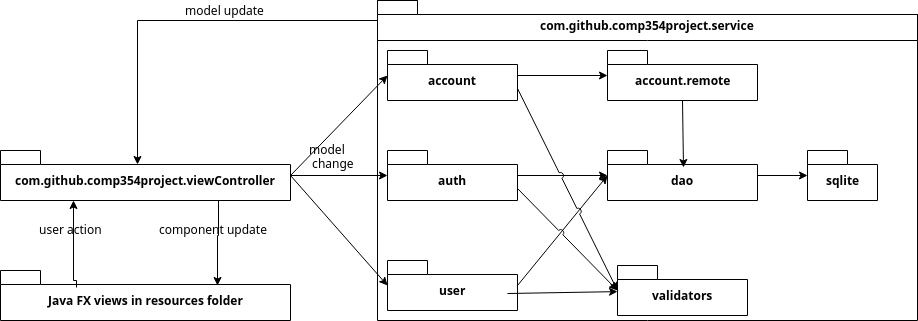
\includegraphics[width=\linewidth]{package-diagram.png}
\end{figure}

The \textit{view}, our graphical user interface, is implemented through the JAVAFX front-end framework. It consists of table views, menus, labels and other GUI components, which are then populated by the view controllers with data from the model. The view is the only component that the user interacts with. It reports any user-triggered events (mouse clicks, text entries...) to the view controllers, and renders the updated model received from the controller. A more in-depth view of the interaction between the user and the view can be seen in the dynamic models, in section \ref{Dynamic Models}.

The \textit{controllers}. The controller populates the views with the model and translates user input into service calls to manipulate the model. When the model is changed, it repopulates the views with new data. 

The \textit{model} is consists of two parts: the application logic, and the data. The application logic is organised in a layered structure of services, which each manage a different section of the system (session management, accounts, users, etc).
Each service performs validation related to its system domain on its inputs, and then delegates the calls to the services of the layer below. The Database Access Objects (DAO) lie  at the bottom of the hierarchy and directly communicate with the database. For examples in the controllers, their services, their intercommunication, and their validation, see section \ref{subsystem interface}.
The data is stored in an SQLite database. Our system actually employs two databases; The first, a local database, and the second, a "remote" database (also local, but acts as if it were remote) used to simulate the bank servers. The data itself consists of model classes, (e.g. bank account, account transaction, user account), which corresponds to the domain model of our application. See section \ref{subsystem interface} for more details on these services and the databases.


\subsection{Subsystem Interface Specifications} \label{subsystem interface}

%VIEW -----------
\subsubsection*{View Subsystem}
\begin{figure}[H]
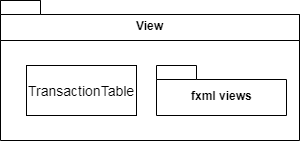
\includegraphics[width=\linewidth]{view_subsystem.png}
\end{figure}
Our resources/fxml folder contains the view subsystem. The view is implemented, as mentioned before, through the JavaFX framework. It is a collection of FXML files, containing a structure contained in an AnchorPane. If the view model is simple menu (Login.fxml, SignUp.fxml, UpdateUserAccount.fxml), it will merely contain a few labeled text fields and buttons with 'onAction' parameters tying the buttons to a function in the view controllers. If it is a table view, (AccountDetails.fxml, AccountList.fxml, AllTransactions.fxml), then a TableView will be used with labelled columns, which are then recognised by the controllers in order to populate them with the model data. As nothing in our view contains actual code,  no functions are mentioned here. 

\subsubsection*{Controller Subsystem}

\begin{figure}[H]
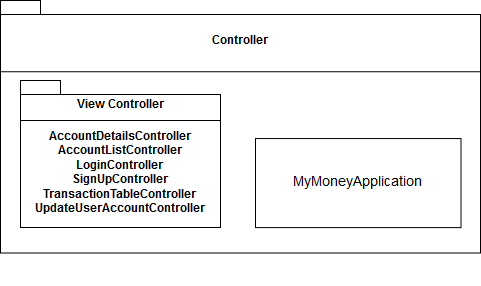
\includegraphics[width=\linewidth]{controller_subsystem.png}
\end{figure}
The com.github.comp354project.viewController package contains a number of controllers for each different view. Each view is handled by its own controller, which contains each column and/or label as a private data member, and each button 'onAction' as a function. All controllers implement the Initializable interface, and hence contain an initialize(URL location, ResourceBundle resources) function which is called when the view is first displayed to the user. This function serves to populate the views with the domain data, if needed.  The controllers may receive user input from the view and catch user events such as button presses or table entry selections. The functions catching these inputs pass these calls to the services in the model, described below.   They are also the ones who pass any errors from the services to the views, mostly to be used for testing and alerting the user of any problems that might have occured.
 A more precise description of each controller is available in \ref{classes}
 
 \subsubsection*{Model Subsystem}
\begin{figure}[H]
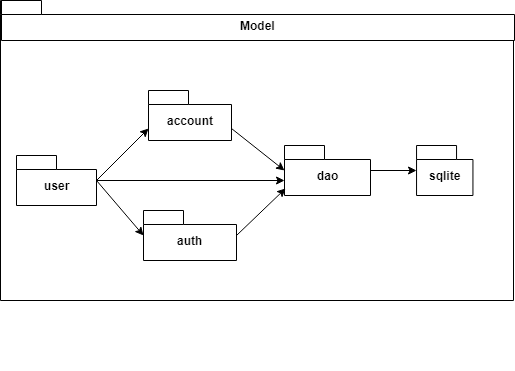
\includegraphics[width=\linewidth]{model_subsystem.png}
\end{figure}
The com.github.comp354project.model package contains both our application logic and our database.  As mentioned in the previous section, it is organised in a layered manner, wherein each layer handles its own services and use the services of the layer below it within worrying about that layer's implementation. Data validation and processing is offered by each service: The account service, for example, validate calls to add or delete bank accounts, edit a transaction's category, or query for specific accounts. It does this by querying the database using an account DAO, and ensuring data integrity and validity (with regards to the business rules). It does not, however, worry about user authorisation, and simply assumes the layer above it (The user service) will have handled it. The com.github.comp354project.viewController calls services within this package to update the view and the model.

The com.github.comp354project.service package.account.remote package is a subsystem to our model which mocks an API call to remote servers of banks or credit card companies. In our case however, we don't actually have access to such systems. For this reason, the remote data exists in an SQLite database like our local one.

\clearpage

\section{Detailed Design} \label{sec:detail}

The myMoney system architecture is designed to be easily modified because of the low coupling between the modules. This was done with interfaces and auto injection of dependencies in classes. Each service package has a Module class designed to bind and provide an implementation to an interface. This way, classes are never instantiated directly into each other, but injected. This design pattern is useful because a change in implementation is as simple as creating a new class and change the module binding. The classes that use it and the tests should in no way be changed. Mocking classes for test purposes is also much easier.

As a side note, we noticed that merge conflicts using git were much less likely to happen because we can each work on different parts of the system without modifying another module.

The tool used for this purpose is Dagger version 2.

\subsection{Class Diagram}

In this section we provide the class diagram of our system, useful for the system developers and testers.This is an in depth look at all of the classes within our system see figure \ref{fig:class-diagram} below If a term is unclear, view section \ref{glossary} for the glossary.

\begin{figure}[H]
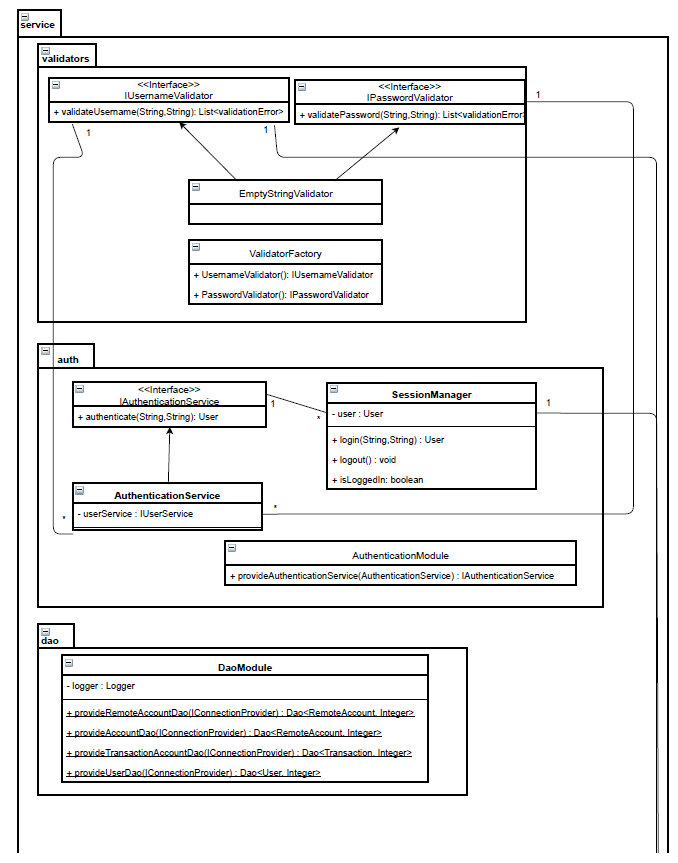
\includegraphics[width=\linewidth]{ClassDiagram1.png}
\end{figure}

\begin{figure}[H]
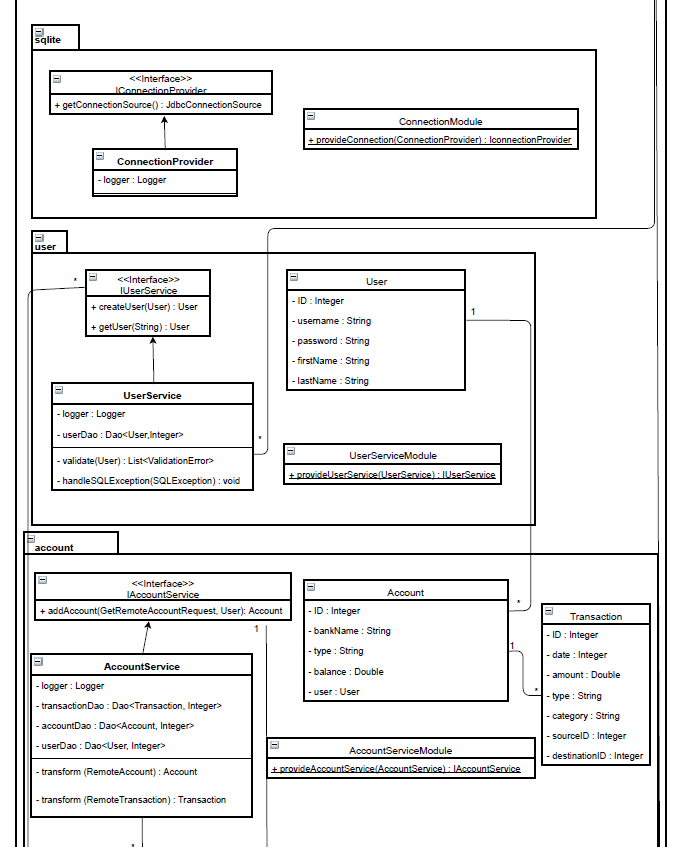
\includegraphics[width=\linewidth]{ClassDiagram2.png}
\end{figure}

\begin{figure}[H]
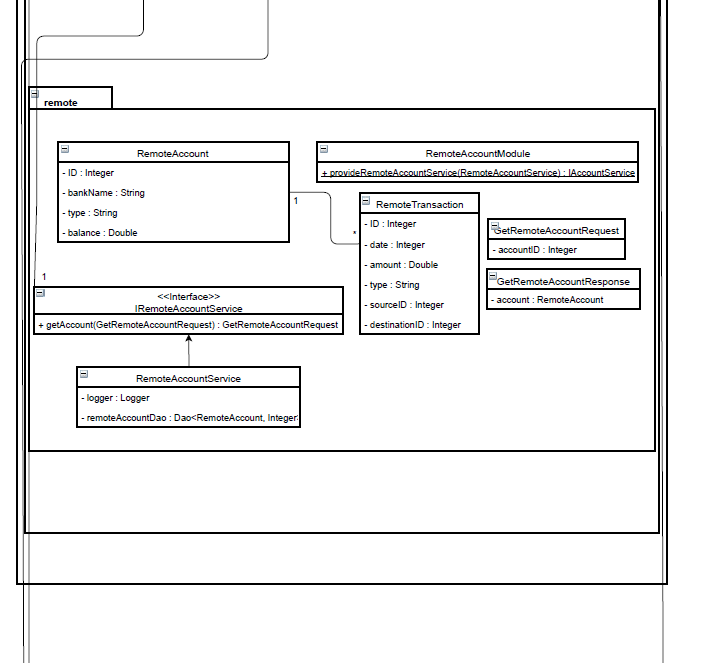
\includegraphics[width=\linewidth]{ClassDiagram3.png}
\end{figure}

\begin{figure}[H]
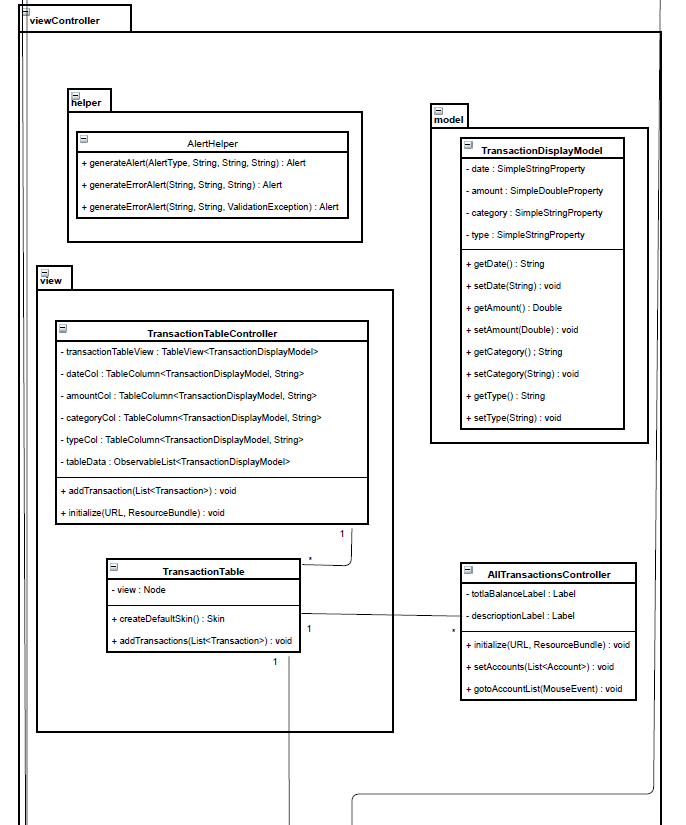
\includegraphics[width=\linewidth]{ClassDiagram4.png}
\end{figure}

\begin{figure}[H]
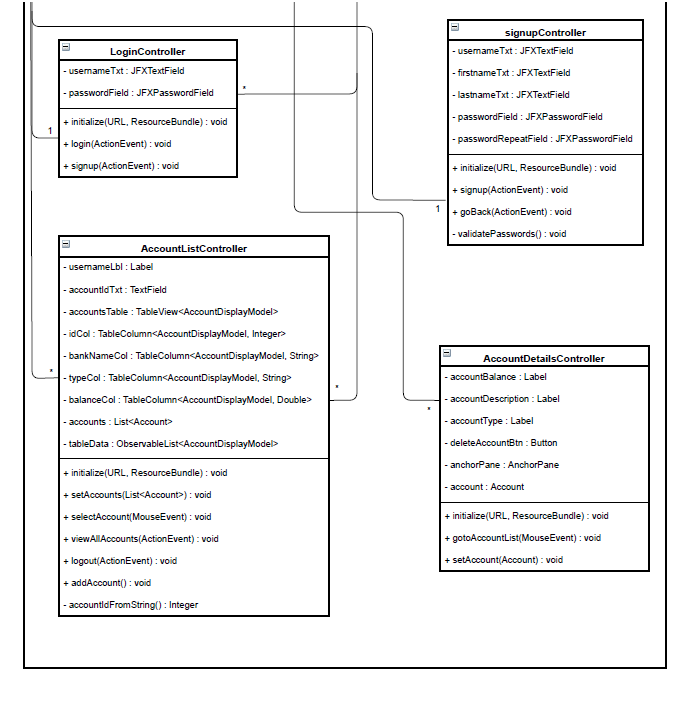
\includegraphics[width=\linewidth]{ClassDiagram5.png}
\caption{Class Diagram}
\label{fig:class-diagram}
\end{figure}

\clearpage

\subsection{Classes}\label{classes}

%Start of com.github.comp354project%
\begin{table}[H]
\centering
\caption{Interface ApplicationComponent}
\resizebox{\textwidth}{!}{%
\begin{tabular}{|l|l|l|l|l|}
\hline
\textbf{Class Name}               & \multicolumn{4}{l|}{com.github.comp354project.ApplicationComponent}                                                                                            \\ \hline
\textbf{Visibility}        & \multicolumn{4}{l|}{Public}   \\ \hline
\textbf{Type}                     & \multicolumn{4}{l|}{Interface}                                                                                                                                 \\ \hline
\textbf{Inherits}                 & \multicolumn{4}{l|}{N/A}                                                                                                                                       \\ \hline
\textbf{Implements}               & \multicolumn{4}{l|}{N/A}                                                                                                                                       \\ \hline
\textbf{Description}              & \multicolumn{4}{l|}{Class dependencies can be injected into the classes defined in the inject methods. This class is used for the Dagger2 injection framework} \\ \hline
\textbf{Attributes}               & \textbf{Visibility}   & \textbf{Data Type}                                                & \textbf{Name}      & \textbf{Description}                          \\ \hline
None                              &                       &                                                                   &                    &                                               \\ \hline
\multirow{7}{*}{\textbf{Methods}} & \textbf{Visibility}   & \textbf{Name}                                                     & \textbf{Returns}   & \textbf{Description}                          \\ \cline{2-5}
                                  & public                & inject(MyMoneyApplication myMoneyApplication)                     & void               & \begin{tabular}[c]{@{}l@{}}Injector for \\ MyMoneyApplication class \end{tabular}        \\ \cline{2-5}
                                  & public                & inject(LoginController loginController)                           & void               & \begin{tabular}[c]{@{}l@{}}Injector for \\ the LoginController class\end{tabular}        \\ \cline{2-5}
                                  & public                & inject(AccountListController accountListController)               & void               & \begin{tabular}[c]{@{}l@{}}Injector for \\ the AccountListController class\end{tabular}  \\ \cline{2-5}
                                  & public                & inject(SignUpController signUpController)                         & void               & \begin{tabular}[c]{@{}l@{}}Injector for \\ the SignUpController class\end{tabular}             \\ \cline{2-5}
                                  & public                & inject(TransactionTableController tableController)                & void               & \begin{tabular}[c]{@{}l@{}}Injector for \\ the TransactionTableController \\ class\end{tabular}   \\ \cline{2-5}
                                  & public                & inject(UpdateUserAccountController updateUserAccountController)   & void               & \begin{tabular}[c]{@{}l@{}}Injector for \\ the UpdateUserAccountController \\ class\end{tabular}  \\ \hline
\end{tabular}
}
\end{table}

\begin{table}[H]
\centering
\caption{Class BusinessRulesConstants}
\resizebox{\textwidth}{!}{%
\begin{tabular}{|l|l|l|l|l|}
\hline
\textbf{Class Name}  & \multicolumn{4}{l|}{com.github.comp354project.BusinessRulesConstants}                               \\ \hline
\textbf{Visibility}        & \multicolumn{4}{l|}{Public}   \\ \hline
\textbf{Type}        & \multicolumn{4}{l|}{Class}                                                                          \\ \hline
\textbf{Inherits}    & \multicolumn{4}{l|}{N/A}                                                                            \\ \hline
\textbf{Implements}  & \multicolumn{4}{l|}{N/A}                                                                            \\ \hline
\textbf{Description} & \multicolumn{4}{l|}{Contains business rules configuration for validators}                           \\ \hline
\textbf{Attributes}  & \textbf{Visibility} & \textbf{Data Type} & \textbf{Name}         & \textbf{Description}             \\ \hline
                     & public              & Integer            & USERNAME\_MIN\_LENGTH & The minimum length of a username \\ \hline
                     & public              & Integer            & USERNAME\_MAX\_LENGTH & The maximum length of a username \\ \hline
                     & public              & Integer            & PASSWORD\_MIN\_LENGTH & The minimum length of a password \\ \hline
                     & public              & Integer            & PASSWORD\_MAX\_LENGTH & The maximum length of a password \\ \hline
                     & public              & Integer            & CATEGORY\_MIN\_LENGTH & The minimum length of a category \\ \hline
                     & public              & Integer            & CATEGORY\_MAX\_LENGTH & The maximum length of a category \\ \hline
\textbf{Methods}     & \textbf{Visibility} & \textbf{Name}      & \textbf{Returns}      & \textbf{Description}             \\ \hline
None                 &                     &                    &                       &                                  \\ \hline
\end{tabular}
}
\end{table}

\begin{table}[H]
\centering
\caption{Class Main}
\begin{tabular}{|l|l|l|l|l|}
\hline
\textbf{Class Name}  & \multicolumn{4}{l|}{com.github.comp354project.Main}                                                                                              \\ \hline
\textbf{Visibility}        & \multicolumn{4}{l|}{Public}   \\ \hline
\textbf{Type}        & \multicolumn{4}{l|}{Class}                                                                                                                       \\ \hline
\textbf{Inherits}    & \multicolumn{4}{l|}{N/A}                                                                                                                         \\ \hline
\textbf{Implements}  & \multicolumn{4}{l|}{N/A}                                                                                                                         \\ \hline
\textbf{Description} & \multicolumn{4}{l|}{Launches the application}                                                                                                    \\ \hline
\textbf{Attributes}  & \textbf{Visibility} & \textbf{Data Type}      & \textbf{Name}    & \textbf{Description}                                                          \\ \hline
None                 &                     &                         &                  &                                                                               \\ \hline
\textbf{Methods}     & \textbf{Visibility} & \textbf{Name}           & \textbf{Returns} & \textbf{Description}                                                          \\ \hline
                     & public              & main(String{[}{]} args) & void             & \begin{tabular}[c]{@{}l@{}}The entry point of \\ the application\end{tabular} \\ \hline
\end{tabular}
\end{table}


\begin{table}[H]
\centering
\caption{Class MyMoneyApplication}
\resizebox{\textwidth}{!}{%
\begin{tabular}{|l|l|l|l|l|}
\hline
\textbf{Class Name}  & \multicolumn{4}{l|}{com.github.comp354project.MyMoneyApplication}                                                                                                                                                                         \\ \hline
\textbf{Visibility}        & \multicolumn{4}{l|}{Public}   \\ \hline
\textbf{Type}        & \multicolumn{4}{l|}{Class}                                                                                                                                                                                                                \\ \hline
\textbf{Inherits}    & \multicolumn{4}{l|}{Application}                                                                                                                                                                                                          \\ \hline
\textbf{Implements}  & \multicolumn{4}{l|}{N/A}                                                                                                                                                                                                                  \\ \hline
\textbf{Description} & \multicolumn{4}{l|}{Entry point for the GUI of the application}                                                                                                                                                                           \\ \hline
\textbf{Attributes}  & \textbf{Visibility} & \textbf{Data Type}                                            & \textbf{Name}      & \textbf{Description}                                                                                                           \\ \hline
                     & private             & Logger                                                        & logger             & Logs event information                                                                                                         \\ \hline
                     & public              & MyMoneyApplication                                            & application        & The GUI entry point variable                                                                                                   \\ \hline
                     & protected           & SessionManager                                                & sessionManager     & Manages user sessions                                                                                                          \\ \hline
                     & private             & ApplicationComponent                                          & component          & Used to instantiate and inject classes                                                                                         \\ \hline
                     & private             & Stage                                                         & primaryStage       & Used to display the GUI                                                                                                        \\ \hline
\textbf{Methods}     & \textbf{Visibility} & \textbf{Name}                                                 & \textbf{Returns}   & \textbf{Description}                                                                                                           \\ \hline
                     & public              & MyMoneyApplication                                            & MyMoneyApplication & \begin{tabular}[c]{@{}l@{}}Constructs the class. \\ Initializes an ApplicationComponent\\ for depedency injection\end{tabular} \\ \hline
                     & public              & getScene()                                                    & Scene              & Returns the current scene                                                                                                      \\ \hline
                     & public              & start(Stage primaryStage)                                     & void               & \begin{tabular}[c]{@{}l@{}}Displays the first GUI\\ when the application\\ launches\end{tabular}                               \\ \hline
                     & private             & updateStage(String fxml, String title, int width, int height) & T                  & Updates the current view                                                                                                       \\ \hline
                     & private             & setStageTitle(String title)                                   & void               & Sets the view's title                                                                                                          \\ \hline
                     & public              & displayLogin()                                                & void               & \begin{tabular}[c]{@{}l@{}}Displays the login view\end{tabular}                                                                                            \\ \hline
                     & public              & displaySignUp()                                               & void               & \begin{tabular}[c]{@{}l@{}}Displays the sign up view \end{tabular}                                                                                            \\ \hline
                     & public              & displayAccounts()                                             & void               & \begin{tabular}[c]{@{}l@{}}Displays the user accounts view \end{tabular}                                                                                            \\ \hline
                     & public              & displayUpdateUser()                                           & void               & \begin{tabular}[c]{@{}l@{}}Displays the update user view \end{tabular}                                                                                            \\ \hline
                     & public              & displayAccountDetails(Account account)                        & void               & \begin{tabular}[c]{@{}l@{}}Displays the account details view \end{tabular}                                                                                            \\ \hline
                     & public              & displayAllTransactions(List accounts)                       & void               & \begin{tabular}[c]{@{}l@{}}Displays all transactions details view \end{tabular}                                                                                            \\ \hline
\end{tabular}%
}
\end{table}
%End of com.github.comp354project%

%Start of com.github.comp354project.service.user
\begin{table}[]
    \centering
    \caption{Interface IUserService}
    \resizebox{\textwidth}{!}{%
    \begin{tabular}{|l|l|l|l|l|}
    \hline
    Class Name & \multicolumn{4}{l|}{com.github.comp345project.model.user.IUserService}                             \\ \hline
    Type       & \multicolumn{4}{l|}{Interface}                                                                        \\ \hline
    Inherits   & \multicolumn{4}{l|}{N/A}                                                                              \\ \hline
    Implements & \multicolumn{4}{l|}{N/A}                                                                              \\ \hline
    Attributes & Visibility  & Data Type                          & Name    & Description                              \\ \hline
                & N/A         &                                    &         &                                          \\ \hline
    Method     & Visibility  & Name                               & Returns & Description                              \\ \hline
                & no modifier & createUser(User user)              & User    & User to create a new user                \\ \hline
                & no modifier & deleteBankAccount(Account account) & void    & Deletes a bank account belonging to user \\ \hline
                & no modifier & updateUser(User user)              & User    & Updates the user's info                  \\ \hline
                & no modifier & deleteUser(User user)              & void    & Deletes a user                           \\ \hline
    \end{tabular}
    }
    \end{table}
    
    \begin{table}[]
    \centering
    \caption{Class User}
    \resizebox{\textwidth}{!}{%
    \begin{tabular}{|l|l|l|l|l|}
    \hline
    Class Name & \multicolumn{4}{l|}{com.github.comp345project.model.user.User}       \\ \hline
    Type       & \multicolumn{4}{l|}{Class}                                              \\ \hline
    Inherits   & \multicolumn{4}{l|}{N/A}                                                \\ \hline
    Implements & \multicolumn{4}{l|}{N/A}                                                \\ \hline
    Attributes & Visibility & Data Type         & Name      & Description                \\ \hline
                & private    & Integer           & ID        & User identification number \\ \hline
                & private    & String            & username  & Username of user           \\ \hline
                & private    & String            & password  & User's password            \\ \hline
                & private    & String            & firstName & User's first name          \\ \hline
                & private    & String            & lastName  & User's last name           \\ \hline
                & private    & String            & email     & User's email               \\ \hline
                & private    & String            & address   & User's address             \\ \hline
                & private    & String            & phone     & User's phone number        \\ \hline
                & private    & ForeignCollection & accounts  & Accounts belonging to user \\ \hline
    Method     & Visibility & Name              & Returns   & Description                \\ \hline
                & N/A        &                   &           &                            \\ \hline
    \end{tabular}
    }
    \end{table}
    
    \begin{table}[]
    \centering
    \caption{Class UserService}
    \resizebox{\textwidth}{!}{%
    \begin{tabular}{|l|l|l|l|l|}
    \hline
    Class Name & \multicolumn{4}{l|}{com.github.comp345project.model.user.UserService}                                                                                                                                                         \\ \hline
    Type       & \multicolumn{4}{l|}{Class}                                                                                                                                                                                                    \\ \hline
    Inherits   & \multicolumn{4}{l|}{N/A}                                                                                                                                                                                                          \\ \hline
    Implements & \multicolumn{4}{l|}{IUserService}                                                                                                                                                                                                          \\ \hline
    Attributes & Visibility & Data Type                                                                                             & Name              & Description                                                                              \\ \hline
                & Private    & Logger                                                                                                & logger            & Logger used to Log things such as errors                                                 \\ \hline
                & Private    & Dao                                                                                                   & userDao           & User data access object used to interact with the user data stored in the database       \\ \hline
                & Private    & Dao                                                                                                   & accountDao        & Account data access object used to interact with the account data stored in the database \\ \hline
                & Private    & IUsernameValidator                                                                                    & usernameValidator & Used to validate a username                                                              \\ \hline
                & Private    & IUserValidator                                                                                        & userValidator     & Used to validate a user                                                                  \\ \hline
                & Private    & SessionManager                                                                                        & sessionManager    & Used to keep track of the currently logged in user                                       \\ \hline
                & Private    & AccountService                                                                                        & accountService    & Used to interact with the account service layer                                          \\ \hline
    Method     & Visibility & Name                                                                                                  & Returns           & Description                                                                              \\ \hline
                & public     & UserService(Dao userDao,Dao accountDao, SessionManager sessionManager, AccountService accountService) & N/A               & constructor used to create UserService                                                   \\ \hline
                & public     & createUser(User user)                                                                                 & User              & User to create a new user                                                                \\ \hline
                & public     & getUser(String username)                                                                              & User              & Get's a user by their username                                                           \\ \hline
                & public     & deleteBankAccount(Account account)                                                                    & void              & Deletes a bank account belonging to user                                                 \\ \hline
                & public     & updateUser(User user)                                                                                 & User              & Updates the user's info                                                                  \\ \hline
                & public     & deleteUser(User user)                                                                                 & void              & Deletes a user                                                                           \\ \hline
    \end{tabular}
    }
    \end{table}
    
    \begin{table}[]
    \centering
    \caption{Class UserServiceModule}
    \resizebox{\textwidth}{!}{%
    \begin{tabular}{|l|l|l|l|l|}
    \hline
    Class Name & \multicolumn{4}{l|}{com.github.comp345project.model.user.UserServiceModule}                   \\ \hline
    Type       & \multicolumn{4}{l|}{Class}                                                                       \\ \hline
    Inherits   & \multicolumn{4}{l|}{N/A}                                                                         \\ \hline
    Implements & \multicolumn{4}{l|}{N/A}                                                                         \\ \hline
    Attributes & Visibility & Data Type                                   & Name         & Description            \\ \hline
                & N/A        &                                             &              &                        \\ \hline
    Method     & Visibility & Name                                        & Returns      & Description            \\ \hline
                & public     & provideUserService(UserService userService) & IUserService & Provides a UserService \\ \hline
    \end{tabular}
    }
    \end{table}
    %Start of com.github.comp354project.service.user
    
    %Start of com.github.comp354project.model.validators
    \begin{table}[]
    \centering
    \caption{Interface ICategoryNameValidator}
    \resizebox{\textwidth}{!}{%
    \begin{tabular}{|l|l|l|l|l|}
    \hline
    Class Name & \multicolumn{4}{l|}{com.github.comp345project.model.validators.ICategoryNameValidator} \\ \hline
    Type & \multicolumn{4}{l|}{Interface} \\ \hline
    Inherits & \multicolumn{4}{l|}{N/A} \\ \hline
    Implements & \multicolumn{4}{l|}{N/A} \\ \hline
    Attributes & Visibility & Data Type & Name & Description \\ \hline
        & N/A &  &  &  \\ \hline
    Method & Visibility & Name & Returns & Description \\ \hline
        & public & validateCategory(String category, String message) & List & Validates transaction categories \\ \hline
    \end{tabular}
    }
    \end{table}
    
    \begin{table}[]
    \centering
    \caption{Interface INameValidator}
    \resizebox{\textwidth}{!}{%
    \begin{tabular}{|l|l|l|l|l|}
    \hline
    Class Name & \multicolumn{4}{l|}{com.github.comp345project.model.validators.INameValidator} \\ \hline
    Type & \multicolumn{4}{l|}{Interface} \\ \hline
    Inherits & \multicolumn{4}{l|}{N/A} \\ \hline
    Implements & \multicolumn{4}{l|}{N/A} \\ \hline
    Attributes & Visibility & Data Type & Name & Description \\ \hline
        & N/A &  &  &  \\ \hline
    Method & Visibility & Name & Returns & Description \\ \hline
        & public & validateName(String name, String message) & List & Validates first and last name of user \\ \hline
    \end{tabular}
    }
    \end{table}
    
    \begin{table}[]
    \centering
    \caption{Interface INameValidator}
    \resizebox{\textwidth}{!}{%
    \begin{tabular}{|l|l|l|l|l|}
    \hline
    Class Name & \multicolumn{4}{l|}{com.github.comp345project.model.validators.INameValidator} \\ \hline
    Type & \multicolumn{4}{l|}{Interface} \\ \hline
    Inherits & \multicolumn{4}{l|}{N/A} \\ \hline
    Implements & \multicolumn{4}{l|}{N/A} \\ \hline
    Attributes & Visibility & Data Type & Name & Description \\ \hline
        & N/A &  &  &  \\ \hline
    Method & Visibility & Name & Returns & Description \\ \hline
        & public & validatePassword(String password, String message) & List & Validates that password meets required criteria \\ \hline
    \end{tabular}
    }
    \end{table}
    
    \begin{table}[]
    \centering
    \caption{Interface INameValidator}
    \resizebox{\textwidth}{!}{%
    \begin{tabular}{|l|l|l|l|l|}
    \hline
    Class Name & \multicolumn{4}{l|}{com.github.comp345project.model.validators.INameValidator} \\ \hline
    Type & \multicolumn{4}{l|}{Interface} \\ \hline
    Inherits & \multicolumn{4}{l|}{N/A} \\ \hline
    Implements & \multicolumn{4}{l|}{N/A} \\ \hline
    Attributes & Visibility & Data Type & Name & Description \\ \hline
        & N/A &  &  &  \\ \hline
    Method & Visibility & Name & Returns & Description \\ \hline
        & public & validateUsername(String username, String message) & List & Validates that username meets required criteria \\ \hline
    \end{tabular}
    }
    \end{table}
    
    \begin{table}[]
    \centering
    \caption{Interface IUserValidator}
    \resizebox{\textwidth}{!}{%
    \begin{tabular}{|l|l|l|l|l|}
    \hline
    Class Name & \multicolumn{4}{l|}{com.github.comp345project.model.validators.IUserValidator} \\ \hline
    Type & \multicolumn{4}{l|}{Interface} \\ \hline
    Inherits & \multicolumn{4}{l|}{N/A} \\ \hline
    Implements & \multicolumn{4}{l|}{N/A} \\ \hline
    Attributes & Visibility & Data Type & Name & Description \\ \hline
        & N/A &  &  &  \\ \hline
    Method & Visibility & Name & Returns & Description \\ \hline
        & public & validateUser(User user) & List & Validates the user data \\ \hline
    \end{tabular}
    }
    \end{table}
    
    \begin{table}[]
    \centering
    \caption{Class StringLengthValidator}
    \resizebox{\textwidth}{!}{%
    \begin{tabular}{|l|l|l|l|l|}
    \hline
    Class Name & \multicolumn{4}{l|}{com.github.comp345project.model.validators.StringLengthValidator} \\ \hline
    Type & \multicolumn{4}{l|}{Class} \\ \hline
    Inherits & \multicolumn{4}{l|}{ICategoryNameValidator, IUsernameValidator, IPasswordValidator, INameValidator} \\ \hline
    Implements & \multicolumn{4}{l|}{N/A} \\ \hline
    Attributes & Visibility & Data Type & Name & Description \\ \hline
        & private & Integer & minLength & Minimum length of String \\ \hline
        & private & Integer & maxLength & Maximum length of String \\ \hline
    Method & Visibility & Name & Returns & Description \\ \hline
        & public & StringLengthValidator(intminLength, int maxLength) & N/A & constructor \\ \hline
        & public & validateName(String name, String message) & List & validates first and last name of user \\ \hline
        & public & validateCategory(String category, String message) & List & validates the category of a transaction \\ \hline
        & public & validatePassword(String password, String message) & List & validates that password meets criteria \\ \hline
        & public & validateUsername(String username, String message) & List & validates that username meets criteria \\ \hline
        & public & validate(String string, String paramName, String message) & List & validates the length of a string \\ \hline
    \end{tabular}%
    }
    \end{table}
    
    \begin{table}[]
    \centering
    \caption{Class UserValidator}
    \resizebox{\textwidth}{!}{%
    \begin{tabular}{|l|l|l|l|l|}
    \hline
    Class Name & \multicolumn{4}{l|}{com.github.comp345project.model.validators.UserValidator} \\ \hline
    Type & \multicolumn{4}{l|}{Class} \\ \hline
    Inherits & \multicolumn{4}{l|}{IUserValidator} \\ \hline
    Implements & \multicolumn{4}{l|}{N/A} \\ \hline
    Attributes & Visibility & Data Type & Name & Description \\ \hline
        & private & IUsernameValidator & usernameValidator & used to validate the user \\ \hline
        & private & IPasswordValidator & passwordValidator & used to validate the user's password \\ \hline
        & private & INameValidator & nameValidator & used to validate the first and last name of user \\ \hline
    Method & Visibility & Name & Returns & Description \\ \hline
        & public & \begin{tabular}[c]{@{}l@{}}UserValidator(IUsernameValidatorusernameValidator, IPasswordValidator \\ passwordValidator, INameValidator nameValidator)\end{tabular} & N/A & Constructor \\ \hline
        & public & validateUser(Useruser) & List & validates user attributes \\ \hline
    \end{tabular}%
    }
    \end{table}
    
    \begin{table}[]
    \centering
    \caption{Class ValidatorFactory}
    \resizebox{\textwidth}{!}{%
    \begin{tabular}{|l|l|l|l|l|}
    \hline
    Class Name & \multicolumn{4}{l|}{com.github.comp345project.model.validators.ValidatorFactory} \\ \hline
    Type & \multicolumn{4}{l|}{Class} \\ \hline
    Inherits & \multicolumn{4}{l|}{N/A} \\ \hline
    Implements & \multicolumn{4}{l|}{N/A} \\ \hline
    Attributes & Visibility & Data Type & Name & Description \\ \hline
        & N/A &  &  &  \\ \hline
    Method & Visibility & Name & Returns & Description \\ \hline
        & public & usernameValidator() & IUsernameValidator & creates a UsernameValidator \\ \hline
        & public & passwordValidator() & IPasswordValidator & createsa PasswordValidator \\ \hline
        & public & categoryNameValidator() & ICategoryNameValidator & creates a CategoryNameValidato \\ \hline
        & public & userValidator() & IUserValidator & creates a UserValidator \\ \hline
    \end{tabular}%
    }
    \end{table}
    %End of com.github.comp354project.model.validators

%Start of com.github.comp354project.service.account

\begin{table}[H]
\centering
\caption{Class Account}
\resizebox{\textwidth}{!}{%
\begin{tabular}{|l|l|l|l|l|}
\hline
\textbf{Class Name}                  & \multicolumn{4}{l|}{com.github.comp354project.model.account.Account}                                                                             \\ \hline
\textbf{Visibility}        & \multicolumn{4}{l|}{Public}   \\ \hline
\textbf{Type}                        & \multicolumn{4}{l|}{Class}                                                                                                                \\ \hline
\textbf{Inherits}                    & \multicolumn{4}{l|}{N/A}                                                                                                                   \\ \hline
\textbf{Implements}                  & \multicolumn{4}{l|}{N/A}                                                                                                                   \\ \hline
\textbf{Description}                 & \multicolumn{4}{l|}{Used to hold the account information of the user}                                                                      \\ \hline
\multirow{6}{*}{\textbf{Attributes}} & \textbf{Visibility} & \textbf{Data Type}                                & \textbf{Name}    & \textbf{Description}                          \\ \cline{2-5}
                                     & private             & Integer                                           & ID               & bank account identification number            \\ \cline{2-5}
                                     & private             & String                                            & type             & type of bank account (chequing, savings, ect) \\ \cline{2-5}
                                     & private             & Double                                            & balance          & Amount inside the account                     \\ \cline{2-5}
                                     & private             & User                                              & user             & name of the user                              \\ \cline{2-5}
                                     & private             & ForeignCollection\textless Transaction\textgreater & transactions     & transaction object                            \\ \hline
\multirow{2}{*}{\textbf{Methods}}    & \textbf{Visibility} & \textbf{Name}                                     & \textbf{Returns} & \textbf{Description}                          \\ \cline{2-5}
                                     & none                & none                                              & none             & none                                          \\ \hline
\end{tabular}%
}
\end{table}


\begin{table}[H]
\centering
\caption{Class AccountService}
\resizebox{\textwidth}{!}{%
\begin{tabular}{|l|l|l|l|l|}
\hline
\textbf{Class Name}                  & \multicolumn{4}{l|}{com.github.comp354project.model.account.AccountService}                                                                                                                                   \\ \hline
\textbf{Visibility}        & \multicolumn{4}{l|}{Public}   \\ \hline
\textbf{Type}                        & \multicolumn{4}{l|}{Class}                                                                                                                                                                                     \\ \hline
\textbf{Inherits}                    & \multicolumn{4}{l|}{N/A}                                                                                                                                                                                        \\ \hline
\textbf{Implements}                  & \multicolumn{4}{l|}{IAccountService}                                                                                                                                                                            \\ \hline
\textbf{Description}                 & \multicolumn{4}{l|}{\begin{tabular}[c]{@{}l@{}}Class used to request information from the bank\\ database in order to add or delete an account to myMoney application\end{tabular}}                                                                       \\ \hline
\multirow{5}{*}{\textbf{Attributes}} & \textbf{Visibility} & \textbf{Data Type}                          & \textbf{Name}        & \textbf{Description}                                                                                                 \\ \cline{2-5}
                                     & private             & Logger                                      & logger               & \begin{tabular}[c]{@{}l@{}}logger object attribute used\\ to keep track of events\end{tabular}                                                                 \\ \cline{2-5}
                                     & private             & Dao\textless Transaction,Integer\textgreater & transactionDao       & \begin{tabular}[c]{@{}l@{}}Dao object used to \\query transactions\end{tabular}                                                                                \\ \cline{2-5}
                                     & private             & Dao\textless User,Integer\textgreater        & userDao              & \begin{tabular}[c]{@{}l@{}}Dao object used to \\query users\end{tabular}                                                                             \\ \cline{2-5}
                                     & private             & IRemoteAccountService                       & remoteAccountService & \begin{tabular}[c]{@{}l@{}}Dao object used to \\query remote accounts\end{tabular}                                                                                    \\ \hline
\multirow{5}{*}{\textbf{Methods}}    & \textbf{Visibility} & \textbf{Name}                               & \textbf{Returns}     & \textbf{Description}                                                                                                 \\ \cline{2-5}
                                     & public              & addAccount                                  & Account              & \begin{tabular}[c]{@{}l@{}}method to request bank \\information from the database\end{tabular}                                                                 \\ \cline{2-5}
                                     & public              & deleteAccount                               & void                 & \begin{tabular}[c]{@{}l@{}}method to delete a particular \\account from myMoney application\end{tabular}                                                       \\ \cline{2-5}
                                     & public              & transform                                   & Account              & \begin{tabular}[c]{@{}l@{}}method to create the appropriate \\banking info to display for the myMoney app \\based on the retrieved banking info\end{tabular}     \\ \cline{2-5}
                                     & public              & Transaction                                 & transform            & \begin{tabular}[c]{@{}l@{}}method to create the appropriate \\transaction info to display for the myMoney \\app based on the retrieved banking info\end{tabular} \\ \hline
\end{tabular}%
}
\end{table}



\begin{table}[H]
\centering
\caption{Class AccountServiceModule}
\resizebox{\textwidth}{!}{%
\begin{tabular}{|l|l|l|l|l|}
\hline
\textbf{Class Name}                  & \multicolumn{4}{l|}{com.github.comp354project.model.account.AccountServiceModule}                     \\ \hline
\textbf{Visibility}        & \multicolumn{4}{l|}{Public}   \\ \hline
\textbf{Type}                        & \multicolumn{4}{l|}{Class}                                                                                \\ \hline
\textbf{Inherits}                    & \multicolumn{4}{l|}{N/A}                                                                                \\ \hline
\textbf{Implements}                  & \multicolumn{4}{l|}{N/A}                                                                                \\ \hline
\textbf{Description}                 & \multicolumn{4}{l|}{used to return need objects for account and transaction needs}                      \\ \hline
\multirow{2}{*}{\textbf{Attributes}} & \textbf{Visibility} & \textbf{Data Type}        & \textbf{Name}      & \textbf{Description}             \\ \cline{2-5}
                                     & None                & none                      & none               & none                             \\ \hline
\multirow{3}{*}{\textbf{Methods}}    & \textbf{Visibility} & \textbf{Name}             & \textbf{Returns}   & \textbf{Description}             \\ \cline{2-5}
                                     & public              & provideTransactionService & transactionService & return transactionService Object \\ \cline{2-5}
                                     & public              & provideAccountService     & accountService     & returns accountService Object    \\ \hline
\end{tabular}%
}
\end{table}


\begin{table}[H]
\centering
\caption{Interface IAccountService}
\resizebox{\textwidth}{!}{%
\begin{tabular}{|l|l|l|l|l|}
\hline
\textbf{Class Name}               & \multicolumn{4}{l|}{com.github.comp354project.model.account.IAccountService}     \\ \hline
\textbf{Visibility}        & \multicolumn{4}{l|}{Public}   \\ \hline
\textbf{Type}                     & \multicolumn{4}{l|}{Interface}                                                     \\ \hline
\textbf{Inherits}                 & \multicolumn{4}{l|}{N/A}                                                           \\ \hline
\textbf{Implements}               & \multicolumn{4}{l|}{N/A}                                                           \\ \hline
\textbf{Description}              & \multicolumn{4}{l|}{interface class for adding and deleting an account}            \\ \hline
\textbf{Attributes}               & \textbf{Visibility} & \textbf{Data Type} & \textbf{Name}    & \textbf{Description} \\ \hline
None                              & None                & None               & none             & none                 \\ \hline
\multirow{3}{*}{\textbf{Methods}} & \textbf{Visibility} & \textbf{Name}      & \textbf{Returns} & \textbf{Description} \\ \cline{2-5}
                                  & N/A                 & addAccount         & N/A              & none                 \\ \cline{2-5}
                                  & N/A                 & deleteAccount      & N/A              & none                 \\ \hline
\end{tabular}%
}
\end{table}


\begin{table}[H]
\centering
\caption{Interface ITransactionService}
\resizebox{\textwidth}{!}{%
\begin{tabular}{|l|l|l|l|l|}
\hline
\textbf{Class Name}               & \multicolumn{4}{l|}{com.github.comp354project.model.account.ITransactionService}        \\ \hline
\textbf{Visibility}        & \multicolumn{4}{l|}{Public}   \\ \hline
\textbf{Type}                     & \multicolumn{4}{l|}{Interface}                                                            \\ \hline
\textbf{Inherits}                 & \multicolumn{4}{l|}{N/A}                                                                  \\ \hline
\textbf{Implements}               & \multicolumn{4}{l|}{N/A}                                                                  \\ \hline
\textbf{Description}              & \multicolumn{4}{l|}{interface class to updating transactions based on categories}         \\ \hline
\textbf{Attributes}               & \textbf{Visibility} & \textbf{Data Type}        & \textbf{Name}    & \textbf{Description} \\ \hline
None                              & None                & None                      & None             & None                 \\ \hline
\multirow{2}{*}{\textbf{Methods}} & \textbf{Visibility} & \textbf{Name}             & \textbf{Returns} & \textbf{Description} \\ \cline{2-5}
                                  & N/A                 & updateTransactionCategory & Transaction      & N/A                  \\ \hline
\end{tabular}%
}
\end{table}


\begin{table}[H]
\centering
\caption{Class Transaction}
\resizebox{\textwidth}{!}{%
\begin{tabular}{|l|l|l|l|l|}
\hline
\textbf{Class Name}                  & \multicolumn{4}{l|}{com.github.comp354project.model.account.Transaction}                       \\ \hline
\textbf{Visibility}        & \multicolumn{4}{l|}{Public}   \\ \hline
\textbf{Type}                        & \multicolumn{4}{l|}{Class}                                                                         \\ \hline
\textbf{Inherits}                    & \multicolumn{4}{l|}{N/A}                                                                         \\ \hline
\textbf{Implements}                  & \multicolumn{4}{l|}{N/A}                                                                         \\ \hline
\textbf{Description}                 & \multicolumn{4}{l|}{Class used to contain the attributes needed to hold a transaction's details} \\ \hline
\multirow{8}{*}{\textbf{Attributes}} & \textbf{Visibility}  & \textbf{Data Type}  & \textbf{Name}     & \textbf{Description}            \\ \cline{2-5}
                                     & private              & Integer             & date              & date of a transaction           \\ \cline{2-5}
                                     & private              & Double              & amount            & dollar amount of a transaction  \\ \cline{2-5}
                                     & private              & String              & type              & the type of a transaction       \\ \cline{2-5}
                                     & private              & String              & category          & the category of a transaction   \\ \cline{2-5}
                                     & private              & Integer             & sourceID          & ID number                       \\ \cline{2-5}
                                     & private              & Integer             & destinationID     & ID number                       \\ \cline{2-5}
                                     & private              & Account             & account           & name of the account             \\ \hline
\multirow{2}{*}{\textbf{Methods}}    & \textbf{Visibility}  & \textbf{Name}       & \textbf{Returns}  & \textbf{Description}            \\ \cline{2-5}
                                     & None                 & None                & None              & None                            \\ \hline
\end{tabular}%
}
\end{table}


\begin{table}[H]
\centering
\caption{Class TransactionService}
\resizebox{\textwidth}{!}{%
\begin{tabular}{|l|l|l|l|l|}
\hline
\textbf{Class Name}                  & \multicolumn{4}{l|}{com.github.comp354project.model.account.TransactionService}                                                              \\ \hline
\textbf{Visibility}        & \multicolumn{4}{l|}{Public}   \\ \hline
\textbf{Type}                        & \multicolumn{4}{l|}{Class}                                                                                                                       \\ \hline
\textbf{Inherits}                    & \multicolumn{4}{l|}{N/A}                                                                                                                       \\ \hline
\textbf{Implements}                  & \multicolumn{4}{l|}{ITransactionService}                                                                                                       \\ \hline
\textbf{Description}                 & \multicolumn{4}{l|}{class used to help with transaction changes}                                                                               \\ \hline
\multirow{4}{*}{\textbf{Attributes}} & \textbf{Visibility} & \textbf{Data Type}                          & \textbf{Name}     & \textbf{Description}                                   \\ \cline{2-5}
                                     & private             & Logger                                      & logger            & object used to interact with TransactionService class  \\ \cline{2-5}
                                     & private             & Dao\textless Transaction,Integer\textgreater & transactionDao    & object used to perform methods related to transactions \\ \cline{2-5}
                                     & private             & ICategoryNameValidator                      & categoryValidator & object used to validate if a category is correct       \\ \hline
\multirow{3}{*}{\textbf{Methods}}    & \textbf{Visibility} & \textbf{Name}                               & \textbf{Returns}  & \textbf{Description}                                   \\ \cline{2-5}
                                     & public              & TransactionService                          & N/A               & constructor                                            \\ \cline{2-5}
                                     & public              & updateTransactionCategory                   & Transaction       & used to update a specific transation                   \\ \hline
\end{tabular}%
}
\end{table}

%End of com.github.comp354project.service.account

% Start of com.github.comp354project.service.exception

\begin{table}[H]
\centering
\caption{Class AccountDoesNotExistException}
\resizebox{\textwidth}{!}{%
\begin{tabular}{|l|l|l|l|l|}
\hline
\textbf{Class Name}  & \multicolumn{4}{l|}{com.github.comp354project.model.account.exceptions.AccountDoesNotExistException}                                                             \\ \hline
\textbf{Visibility}        & \multicolumn{4}{l|}{Public}   \\ \hline
\textbf{Type}        & \multicolumn{4}{l|}{class}                                                                                    \\ \hline
\textbf{Inherits}    & \multicolumn{4}{l|}{RuntimeException}                                                                                      \\ \hline
\textbf{Implements}  & \multicolumn{4}{l|}{N/A}                                                                         \\ \hline
\textbf{Description} & \multicolumn{4}{l|}{Exception thrown when a remote account does not exist}                                    \\ \hline
\textbf{Attributes}  & \textbf{Visibility} & \textbf{Data Type}           & \textbf{Name}                & \textbf{Description}      \\ \hline
                     & private             & GetRemoteAccountRequest      & request                      & The request that was sent \\ \hline
\textbf{Methods}     & \textbf{Visibility} & \textbf{Name}                & \textbf{Returns}             & \textbf{Description}      \\ \hline
                     & public              & AccountDoesNotExistException & \begin{tabular}[c]{@{}l@{}}AccountDoesNotExistException(String message, \\Throwable cause, GetRemoteAccountRequest request)\end{tabular} & Constructs the exception  \\ \hline
\end{tabular}%
}
\end{table}

\begin{table}[H]
\centering
\caption{Class AccountExistsException}
\resizebox{\textwidth}{!}{%
\begin{tabular}{|l|l|l|l|l|}
\hline
\textbf{Class Name}  & \multicolumn{4}{l|}{com.github.comp354project.model.account.exceptions.AccountExistsException}                                                       \\ \hline
\textbf{Visibility}        & \multicolumn{4}{l|}{Public}   \\ \hline
\textbf{Type}        & \multicolumn{4}{l|}{class}                                                                        \\ \hline
\textbf{Inherits}    & \multicolumn{4}{l|}{RuntimeException}                                                             \\ \hline
\textbf{Implements}  & \multicolumn{4}{l|}{N/A}                                                                          \\ \hline
\textbf{Description} & \multicolumn{4}{l|}{Exception thrown when an account is already in use}                           \\ \hline
\textbf{Attributes}  & \textbf{Visibility} & \textbf{Data Type}     & \textbf{Name}          & \textbf{Description}      \\ \hline
                     & private             & Account                & account                & The account that was sent \\ \hline
\textbf{Methods}     & \textbf{Visibility} & \textbf{Name}          & \textbf{Returns}       & \textbf{Description}      \\ \hline
                     & public              & AccountExistsException & \begin{tabular}[c]{@{}l@{}}AccountExistsException(String message, \\Throwable cause, Account account)\end{tabular} & Constructs the exception  \\ \hline
\end{tabular}%
}
\end{table}

% End of com.github.comp354project.service.exception

%Start of com.github.comp354project.account.remote

\begin{table}[]
\centering
\caption{Class GetRemoteAccountRequest}
\resizebox{\textwidth}{!}{%
\begin{tabular}{|l|l|l|l|l|l|}
\hline
\textbf{Class Name}  & \multicolumn{5}{l|}{com.github.comp354project.model.account.remote.GetRemoteAccountRequest}                                                                   \\ \hline
\textbf{Visibility}        & \multicolumn{5}{l|}{Public}   \\ \hline
\textbf{Type}        & \multicolumn{5}{l|}{Public}                                                                                    \\ \hline
\textbf{Inherits}    & \multicolumn{5}{l|}{N/A}                                                                                       \\ \hline
\textbf{Implements}  & \multicolumn{5}{l|}{N/A}                                                                                       \\ \hline
\textbf{Description} & \multicolumn{5}{l|}{Retrieve the remote account request}                                                       \\ \hline
\textbf{Attributes}  & \textbf{Visibility} & \textbf{Data Type} & \textbf{Name}    & \multicolumn{2}{l|}{\textbf{Description}}        \\ \hline
                     & Private             & Integer            & accountID        & \multicolumn{2}{l|}{Identification of an account} \\ \hline
\textbf{Methods}     & \textbf{Visibility} & \textbf{Name}      & \textbf{Returns} & \textbf{Description}       & \textbf{Throws}     \\ \hline
None                 &                     &                    &                  &                            &                     \\ \hline
\end{tabular}%
}
\end{table}


\begin{table}[]
\centering
\caption{Class GetRemoteAccountResponse}
\resizebox{\textwidth}{!}{%
\begin{tabular}{|l|l|l|l|l|l|}
\hline
\textbf{Class Name}  & \multicolumn{5}{l|}{com.github.comp354project.model.account.remote.GetRemoteAccountResponse}                                                           \\ \hline
\textbf{Visibility}        & \multicolumn{5}{l|}{Public}   \\ \hline
\textbf{Type}        & \multicolumn{5}{l|}{Public}                                                                             \\ \hline
\textbf{Inherits}    & \multicolumn{5}{l|}{N/A}                                                                                \\ \hline
\textbf{Implements}  & \multicolumn{5}{l|}{N/A}                                                                                \\ \hline
\textbf{Description} & \multicolumn{5}{l|}{Retrieve the response for the remote account request}                               \\ \hline
\textbf{Attributes}  & \textbf{Visibility} & \textbf{Data Type} & \textbf{Name}    & \multicolumn{2}{l|}{\textbf{Description}} \\ \hline
                     & Private             & RemoteAccount      & account          & \multicolumn{2}{l|}{The remote account}   \\ \hline
\textbf{Methods}     & \textbf{Visibility} & \textbf{Name}      & \textbf{Returns} & \textbf{Description}   & \textbf{Throws}  \\ \hline
None                 &                     &                    &                  &                        &                  \\ \hline
\end{tabular}%
}
\end{table}




\begin{table}[]
\centering
\caption{Interface IRemoteAccountService}
\resizebox{\textwidth}{!}{%
\begin{tabular}{|l|l|l|l|l|l|}
\hline
\textbf{Name}        & \multicolumn{5}{l|}{com.github.comp354project.model.account.remote.IRemoteAccountService}                                  \\ \hline
\textbf{Visibility}        & \multicolumn{5}{l|}{Public}   \\ \hline
\textbf{Type}        & \multicolumn{5}{l|}{Public}                                                                                                \\ \hline
\textbf{Inherits}    & \multicolumn{5}{l|}{N/A}                                                                                                   \\ \hline
\textbf{Implements}  & \multicolumn{5}{l|}{N/A}                                                                                                   \\ \hline
\textbf{Description} & \multicolumn{5}{l|}{The interface for the remote account service (request and response)}                                   \\ \hline
\textbf{Attributes}  & \textbf{Visibility}     & \textbf{Data Type}        & \textbf{Name}          & \multicolumn{2}{l|}{\textbf{Description}}   \\ \hline
None                 &                         &                           &                        & \multicolumn{2}{l|}{}                       \\ \hline
\textbf{Methods}     & \textbf{Visibility}     & \textbf{Name}             & \textbf{Throws}        & \multicolumn{2}{l|}{\textbf{Description}}   \\ \hline
                     & Public                  & IRemoteAccountService     & ValidationException    & \multicolumn{2}{l|}{Remote account service} \\ \hline
\end{tabular}%
}
\end{table}



\begin{table}[]
\centering
\caption{Class RemoteAccount}
\label{el}
\resizebox{\textwidth}{!}{%
\begin{tabular}{|l|l|l|l|l|l|}
\hline
\textbf{Class Name}  & \multicolumn{5}{l|}{com.github.comp354project.model.account.remote.RemoteAccount}                            \\ \hline
\textbf{Visibility}        & \multicolumn{5}{l|}{Public}   \\ \hline
\textbf{Type}        & \multicolumn{5}{l|}{Public}                                                                                    \\ \hline
\textbf{Inherits}    & \multicolumn{5}{l|}{N/A}                                                                                       \\ \hline
\textbf{Implements}  & \multicolumn{5}{l|}{N/A}                                                                                       \\ \hline
\textbf{Description} & \multicolumn{5}{l|}{The remote account with details}                                                           \\ \hline
\textbf{Attributes}  & \textbf{Visibility} & \textbf{Data Type} & \textbf{Name}    & \multicolumn{2}{l|}{\textbf{Description}}        \\ \hline
\multirow{5}{*}{}    & Private             & Integer            & ID               & \multicolumn{2}{l|}{ID of the account}           \\ \cline{2-6}
                     & Private             & String             & bankName         & \multicolumn{2}{l|}{Name of the bank}            \\ \cline{2-6}
                     & Private             & String             & Type             & \multicolumn{2}{l|}{Type of the account}         \\ \cline{2-6}
                     & Private             & Double             & balance          & \multicolumn{2}{l|}{Balance of the account}      \\ \cline{2-6}
                     & Private             & ForeignCollection  & transactions     & \multicolumn{2}{l|}{Transactions of the account} \\ \hline
\textbf{Methods}     & \textbf{Visibility} & \textbf{Name}      & \textbf{Returns} & \textbf{Description}       & \textbf{Throws}     \\ \hline
None                 &                     &                    &                  &                            &                     \\ \hline
\end{tabular}%
}
\end{table}



\begin{table}[]
\centering
\caption{Class RemoteAccountModule}

\resizebox{\textwidth}{!}{%
\begin{tabular}{|l|l|l|l|l|}
\hline
\textbf{Class Name}  & \multicolumn{4}{l|}{com.github.comp354project.model.account.remote.RemoteAccountModule}                                                                                    \\ \hline
\textbf{Visibility}        & \multicolumn{4}{l|}{Public}   \\ \hline
\textbf{Type}        & \multicolumn{4}{l|}{Public}                                                                                                                                                  \\ \hline
\textbf{Inherits}    & \multicolumn{4}{l|}{N/A}                                                                                                                                                     \\ \hline
\textbf{Implements}  & \multicolumn{4}{l|}{N/A}                                                                                                                                                     \\ \hline
\textbf{Description} & \multicolumn{4}{l|}{The module for remote account class}                                                                                                                     \\ \hline
\textbf{Attributes}  & \textbf{Visibility}      & \textbf{Data Type}                           & \textbf{Name}                         & \textbf{Description}                                       \\ \hline
None                 &                          &                                              &                                       &                                                            \\ \hline
\textbf{Methods}     & \textbf{Visibility}      & \textbf{Name}                                & \textbf{Returns}                      & \textbf{Description}                                       \\ \hline
\multirow{2}{*}{}    & \multirow{2}{*}{Default} & \multirow{2}{*}{provideRemoteAccountService} & \multirow{2}{*}{remoteAccountService} & \multirow{2}{*}{Module provide the remote account service} \\
                     &                          &                                              &                                       &                                                            \\ \hline
\end{tabular}%
}
\end{table}




\begin{table}[]
\centering
\caption{Class RemoteAccountService}

\resizebox{\textwidth}{!}{%
\begin{tabular}{|l|l|l|l|l|l|}
\hline
\textbf{Class Name}                  & \multicolumn{5}{l|}{com.github.comp354project.model.account.remote.RemoteAccountService}                                                                                                                                                                                                                                                                                                                                              \\ \hline
\textbf{Visibility}        & \multicolumn{4}{l|}{Public}   \\ \hline
\textbf{Type}                        & \multicolumn{5}{l|}{Public}                                                                                                                                                                                                                                                                                                                                                            \\ \hline
\textbf{Inherits}                    & \multicolumn{5}{l|}{N/A}                                                                                                                                                                                                                                                                                                                                                               \\ \hline
\textbf{Implements}                  & \multicolumn{5}{l|}{IRemoteAccountService}                                                                                                                                                                                                                                                                                                                                             \\ \hline
\textbf{Description}                 & \multicolumn{5}{l|}{The services that the remote account can provide}                                                                                                                                                                                                                                                                                                                  \\ \hline
\multirow{2}{*}{\textbf{Attributes}} & \textbf{Visibility}         & \textbf{Data Type}                                                                                            & \textbf{Name}                                                                       & \multicolumn{2}{l|}{\textbf{Description}}                                                                                                          \\ \cline{2-6}
                                     & Private                     & Logger                                                                                                        & logger                                                                              & \multicolumn{2}{l|}{\begin{tabular}[c]{@{}l@{}}Gets the log \\ of the Remote\\ AccountService.class\end{tabular}}                                  \\ \hline
                                     & Private                     & \begin{tabular}[c]{@{}l@{}}Dao \textless Remote\\ Account, Integer \textgreater\end{tabular}                  & \begin{tabular}[c]{@{}l@{}}Remote\\ AccountDao\end{tabular}                         & \multicolumn{2}{l|}{RemoteAccountDoa}                                                                                                              \\ \hline
\textbf{Methods}                     & \textbf{Visibility}         & \textbf{Name}                                                                                                 & \textbf{Throws}                                                                     & \multicolumn{2}{l|}{\textbf{Description}}                                                                                                          \\ \hline
                                     & \multicolumn{1}{c|}{Public} & \multicolumn{1}{c|}{RemoteAccountService(Dao  \textless RemoteAccount,Integer \textgreater remoteAccountDao)} & \multicolumn{1}{c|}{N/A}                                                            & \multicolumn{2}{l|}{\begin{tabular}[c]{@{}l@{}}The constructor \\ class for Remote\\ AccountService\end{tabular}}                                  \\ \hline
                                     & Public                      & getAccount(GetRemoteAccountRequest request)                                                                   & \multicolumn{1}{c|}{\begin{tabular}[c]{@{}c@{}}Validation\\ Exception\end{tabular}} & \multicolumn{2}{l|}{\begin{tabular}[c]{@{}l@{}}Return the account \\ information if \\ there is a request \\ for it and if it exists\end{tabular}} \\ \hline
\end{tabular}%
}
\end{table}



\begin{table}[]
\centering
\caption{Class RemoteTransaction}

\resizebox{\textwidth}{!}{%
\begin{tabular}{|l|l|l|l|l|}
\hline
\textbf{Class Name}                  & \multicolumn{4}{l|}{com.github.comp354project.model.account.remote.RemoteTransaction}                                                                                                                                           \\ \hline
\textbf{Visibility}        & \multicolumn{4}{l|}{Public}   \\ \hline
\textbf{Type}                        & \multicolumn{4}{l|}{Public}                                                                                                                                                      \\ \hline
\textbf{Inherits}                    & \multicolumn{4}{l|}{N/A}                                                                                                                                                         \\ \hline
\textbf{Implements}                  & \multicolumn{4}{l|}{N/A}                                                                                                                                                         \\ \hline
\textbf{Description}                 & \multicolumn{4}{l|}{The remote transaction class}                                                                                                                                \\ \hline
\multirow{3}{*}{\textbf{Attributes}} & \textbf{Visibility} & \textbf{Data Type} & \textbf{Name}    & \textbf{Description}                                                                                               \\ \cline{2-5}
                                     & Private             & Integer            & ID               & \begin{tabular}[c]{@{}l@{}}Identification of the \\ remote transaction\end{tabular}                                \\ \cline{2-5}
                                     & Private             & Integer            & date             & Date of the transaction                                                                                            \\ \hline
                                     & Private             & Double             & amount           & Amount of money transitioned                                                                                       \\ \hline
                                     & Private             & String             & type             & Type of transaction                                                                                                \\ \hline
                                     & Private             & Integer            & SourceID         & \begin{tabular}[c]{@{}l@{}}Identification of the source \\ where the money was originally\\ resided\end{tabular}   \\ \hline
                                     & Private             & Integer            & destinationID    & \begin{tabular}[c]{@{}l@{}}Identification of the destination\\ where the money will be\\ transitioned\end{tabular} \\ \hline
                                     & Private             & Remote             & account          & The main account of the user                                                                                       \\ \hline
\textbf{Methods}                     & \textbf{Visibility} & \textbf{Name}      & \textbf{Returns} & \textbf{Description}                                                                                               \\ \hline
None                                 &                     &                    &                  &                                                                                                                    \\ \hline
\end{tabular}%
}
\end{table}
%end of com.github.comp354project.account.remote

\begin{table}[H]
\centering
\caption{Class AuthenticationModule}
\label{my-label}
\resizebox{\textwidth}{!}{%
\begin{tabular}{|l|l|l|l|l|}
\hline
\textbf{Class Name}  & \multicolumn{4}{l|}{com.github.comp354project.model.auth.AuthenticationModule}                                                                                                                                             \\ \hline
\textbf{Type}        & \multicolumn{4}{l|}{class}                                                                                                                                                                                                 \\ \hline
\textbf{Inherits}    & \multicolumn{4}{l|}{N/A}                                                                                                                                                                                                   \\ \hline
\textbf{Implements}  & \multicolumn{4}{l|}{N/A}                                                                                                                                                                                                   \\ \hline
\textbf{Description} & \multicolumn{4}{l|}{The authentication module to provide the dependencies}                                                                                                                                                 \\ \hline
\textbf{Attributes}  & \textbf{Visibility} & \textbf{Data Type}                                                                                                     & \textbf{Name}          & \textbf{Description}                               \\ \hline
None                 &                     &                                                                                                                        &                        &                                                    \\ \hline
\textbf{Methods}     & \textbf{Visibility} & \textbf{Name}                                                                                                          & \textbf{Returns}       & \textbf{Description}                               \\ \hline
                     & public              & \begin{tabular}[c]{@{}l@{}}ValidationException(String message, \\ Throwable cause, @Singular List errors)\end{tabular} & IAuthenticationService & Provides the authentication service implementation \\ \hline
\end{tabular}%
}
\end{table}

\begin{table}[H]
\centering
\caption{Class AuthenticationService}
\label{my-label}
\resizebox{\textwidth}{!}{%
\begin{tabular}{|l|l|l|l|l|}
\hline
\textbf{Class Name}  & \multicolumn{4}{l|}{com.github.comp354project.model.auth.AuthenticationService}                                                        \\ \hline
\textbf{Type}        & \multicolumn{4}{l|}{class}                                                                                                             \\ \hline
\textbf{Inherits}    & \multicolumn{4}{l|}{N/A}                                                                                                               \\ \hline
\textbf{Implements}  & \multicolumn{4}{l|}{IAuthenticationService}                                                                                            \\ \hline
\textbf{Description} & \multicolumn{4}{l|}{Service to authenticate users}                                                                                     \\ \hline
\textbf{Attributes}  & \textbf{Visibility} & \textbf{Data Type}                             & \textbf{Name}         & \textbf{Description}                    \\ \hline
                     & private             & Logger                                         & Logger                & Logger                                  \\ \hline
                     & private             & Dao\textless User, Integer\textgreater          & userDao               & The service Dao to interact with the db \\ \hline
                     & private             & IUsernameValidator                             & usernameValidator     & Used to validate a username             \\ \hline
                     & private             & IPasswordValidator                             & passwordValidator     & Used to validate a password             \\ \hline
\textbf{Methods}     & \textbf{Visibility} & \textbf{Name}                                  & \textbf{Returns}      & \textbf{Description}                    \\ \hline
                     & public              & AuthenticationService(Dao userDao)             & AuthenticationService & Constructs an AuthenticationService     \\ \hline
                     & public              & authenticate(String username, String password) & User                  & Authenticates a user                    \\ \hline
                     & private             & getUser(String username)                       & User                  & Finds a user by username                \\ \hline
\end{tabular}%
}
\end{table}

\begin{table}[H]
\centering
\caption{Class IAuthenticationService}
\label{my-label}
\resizebox{\textwidth}{!}{%
\begin{tabular}{|l|l|l|l|l|}
\hline
\textbf{Class Name}  & \multicolumn{4}{l|}{com.github.comp354project.model.auth.IAuthenticationService}                               \\ \hline
\textbf{Type}        & \multicolumn{4}{l|}{Interface}                                                                                 \\ \hline
\textbf{Inherits}    & \multicolumn{4}{l|}{N/A}                                                                                       \\ \hline
\textbf{Implements}  & \multicolumn{4}{l|}{N/A}                                                                                       \\ \hline
\textbf{Description} & \multicolumn{4}{l|}{Service to authenticate users}                                                             \\ \hline
\textbf{Attributes}  & \textbf{Visibility} & \textbf{Data Type}                             & \textbf{Name}    & \textbf{Description} \\ \hline
None                 &                     &                                                &                  &                      \\ \hline
\textbf{Methods}     & \textbf{Visibility} & \textbf{Name}                                  & \textbf{Returns} & \textbf{Description} \\ \hline
                     & public              & authenticate(String username, String password) & User             & Authenticates a user \\ \hline
\end{tabular}%
}
\end{table}

\begin{table}[H]
\centering
\caption{Class SessionManager}
\label{my-label}
\resizebox{\textwidth}{!}{%
\begin{tabular}{|l|l|l|l|l|}
\hline
\textbf{Class Name}  & \multicolumn{4}{l|}{com.github.comp354project.model.auth.SessionManager}                                                                   \\ \hline
\textbf{Type}        & \multicolumn{4}{l|}{Class}                                                                                                                 \\ \hline
\textbf{Inherits}    & \multicolumn{4}{l|}{N/A}                                                                                                                   \\ \hline
\textbf{Implements}  & \multicolumn{4}{l|}{N/A}                                                                                                                   \\ \hline
\textbf{Description} & \multicolumn{4}{l|}{Service to manage user sessions}                                                                                       \\ \hline
\textbf{Attributes}  & \textbf{Visibility} & \textbf{Data Type}                                           & \textbf{Name}         & \textbf{Description}          \\ \hline
                     & private             & IAuthenticationService                                       & authenticationService & The authentication service    \\ \hline
                     & private             & User                                                         & user                  & The current user logged in    \\ \hline
\textbf{Methods}     & \textbf{Visibility} & \textbf{Name}                                                & \textbf{Returns}      & \textbf{Description}          \\ \hline
                     & public              & SessionManager(IAuthenticationService authenticationService) & SessionManager        & Constructs the SessionManager \\ \hline
                     & public              & login(String username, String password)                      & User                  & Authenticates a user          \\ \hline
                     & public              & logout()                                                     & void                  & Disconnects a user            \\ \hline
                     & public              & isLoggedIn()                                                 & boolean               & Checks if a user is logged in \\ \hline
\end{tabular}%
}
\end{table}

% End of com.github.comp354project.model.auth

%Start of com.github.comp354project.auth.exception
\begin{table}[H]
\centering
\caption{Class AuthenticationException}
\resizebox{\textwidth}{!}{%
\begin{tabular}{|l|l|l|l|l|}
\hline
\textbf{Class Name}  & \multicolumn{4}{l|}{com.github.comp354project.model.auth.exceptions.AuthenticationException}                                                                                                                    \\ \hline
\textbf{Visibility}        & \multicolumn{4}{l|}{Public}   \\ \hline
\textbf{Type}        & \multicolumn{4}{l|}{class}                                                                                                                                                                                      \\ \hline
\textbf{Inherits}    & \multicolumn{4}{l|}{Exception}                                                                                                                                                                                  \\ \hline
\textbf{Implements}  & \multicolumn{4}{l|}{N/A}                                                                                                                                                                                        \\ \hline
\textbf{Description} & \multicolumn{4}{l|}{Exception thrown when a user did not authenticate properly}                                                                                                                                 \\ \hline
\textbf{Attributes}  & \textbf{Visibility} & \textbf{Data Type}     & \textbf{Name}                                                                                                                         & \textbf{Description}     \\ \hline
                     & private             & String                 & username                                                                                                                              & The username used        \\ \hline
                     & private             & String                 & password                                                                                                                              & The password used        \\ \hline
\textbf{Methods}     & \textbf{Visibility} & \textbf{Name}          & \textbf{Returns}                                                                                                                      & \textbf{Description}     \\ \hline
                     & public              & AccountExistsException & \begin{tabular}[c]{@{}l@{}}AuthenticationException(String message, Throwable cause, \\ String username, String password)\end{tabular} & Constructs the exception \\ \hline
\end{tabular}%
}
\end{table}

\begin{table}[H]
\centering
\caption{Class AuthorisationException}
\resizebox{\textwidth}{!}{%
\begin{tabular}{|l|l|l|l|l|}
\hline
\textbf{Class Name}  & \multicolumn{4}{l|}{com.github.comp354project.model.auth.exceptions.AuthorisationException}                                                  \\ \hline
\textbf{Visibility}        & \multicolumn{4}{l|}{Public}   \\ \hline
\textbf{Type}        & \multicolumn{4}{l|}{class}                                                                                                                   \\ \hline
\textbf{Inherits}    & \multicolumn{4}{l|}{Exception}                                                                                                               \\ \hline
\textbf{Implements}  & \multicolumn{4}{l|}{N/A}                                                                                                                     \\ \hline
\textbf{Description} & \multicolumn{4}{l|}{Exception thrown when a user is not authorised to execute/read}                                                          \\ \hline
\textbf{Attributes}  & \textbf{Visibility} & \textbf{Data Type}     & \textbf{Name}                                                      & \textbf{Description}     \\ \hline
                     & private             & User                   & user                                                               & The user used            \\ \hline
\textbf{Methods}     & \textbf{Visibility} & \textbf{Name}          & \textbf{Returns}                                                   & \textbf{Description}     \\ \hline
                     & public              & AuthorisationException & AuthorisationException(String message, Throwable cause, User user) & Constructs the exception \\ \hline
\end{tabular}%
}
\end{table}

\begin{table}[H]
\centering
\caption{Class UserLoggedInException}
\resizebox{\textwidth}{!}{%
\begin{tabular}{|l|l|l|l|l|}
\hline
\textbf{Class Name}  & \multicolumn{4}{l|}{com.github.comp354project.model.auth.exceptions.UserLoggedInException}                                                                                            \\ \hline
\textbf{Visibility}        & \multicolumn{4}{l|}{Public}   \\ \hline
\textbf{Type}        & \multicolumn{4}{l|}{class}                                                                                                                                                            \\ \hline
\textbf{Inherits}    & \multicolumn{4}{l|}{Exception}                                                                                                                                                        \\ \hline
\textbf{Implements}  & \multicolumn{4}{l|}{N/A}                                                                                                                                                              \\ \hline
\textbf{Description} & \multicolumn{4}{l|}{Exception thrown when a user needs to be logged in}                                                                                                               \\ \hline
\textbf{Attributes}  & \textbf{Visibility} & \textbf{Data Type}    & \textbf{Name}                                                                                                & \textbf{Description}     \\ \hline
                     & private             & User                  & user                                                                                                         & The user used            \\ \hline
\textbf{Methods}     & \textbf{Visibility} & \textbf{Name}         & \textbf{Returns}                                                                                             & \textbf{Description}     \\ \hline
                     & public              & UserLoggedInException & \begin{tabular}[c]{@{}l@{}}UserLoggedInException(String message, \\ Throwable cause, User user)\end{tabular} & Constructs the exception \\ \hline
\end{tabular}%
}
\end{table}

% End of com.github.comp354project.auth.exception

% Start of com.github.comp354project.service.dao

\begin{table}[H]
\centering
\caption{Class DaoModule}

\resizebox{\textwidth}{!}{%
\begin{tabular}{|l|l|l|l|l|}
\hline
\textbf{Class Name}  & \multicolumn{4}{l|}{com.github.comp354project.model.dao.DaoModule}                                                                                                                                                                 \\ \hline
\textbf{Visibility}        & \multicolumn{4}{l|}{Public}   \\ \hline
\textbf{Type}        & \multicolumn{4}{l|}{Class}                                                                                                                                                                                                           \\ \hline
\textbf{Inherits}    & \multicolumn{4}{l|}{N/A}                                                                                                                                                                                                             \\ \hline
\textbf{Implements}  & \multicolumn{4}{l|}{N/A}                                                                                                                                                                                                             \\ \hline
\textbf{Description} & \multicolumn{4}{l|}{DAO module to bind interfaces to their interfaces and provide them to the classes that require them}                                                                                                             \\ \hline
\textbf{Attributes}  & \textbf{Visibility} & \textbf{Data Type}                                              & \textbf{Name}                                  & \textbf{Description}                                                                        \\ \hline
                     & private             & Logger                                                          & logger                                         & Logs event information                                                                      \\ \hline
\textbf{Methods}     & \textbf{Visibility} & \textbf{Name}                                                   & \textbf{Returns}                               & \textbf{Description}                                                                        \\ \hline
                     & public              & provideRemoteAccountDao(IConnectionProvider connectionProvider) & Dao\textless RemoteAccount, Integer\textgreater & \begin{tabular}[c]{@{}l@{}}Returns the implementation \\ of a RemoteAccountDao\end{tabular} \\ \hline
                     & public              & provideAccountDao(IConnectionProvider connectionProvider)       & Dao\textless Account, Integer\textgreater       & \begin{tabular}[c]{@{}l@{}}Returns the implementation\\ of an AccountDao\end{tabular}       \\ \hline
                     & public              & provideTransactionDao(IConnectionProvider connectionProvider)   & Dao\textless Transaction, Integer\textgreater   & \begin{tabular}[c]{@{}l@{}}Returns the implementation\\ of a TransactionDao\end{tabular}    \\ \hline
                     & public              & provideUserDao(IConnectionProvider connectionProvider)          & Dao\textless User, Integer\textgreater          & \begin{tabular}[c]{@{}l@{}}Returns the implementation\\ of a UserDao\end{tabular}           \\ \hline
\end{tabular}%
}
\end{table}

%end of com.github.comp354project.service.dao

%start of com.github.comp354project.model.exceptions

\begin{table}[H]
\centering
\caption{Class UserLoggedInException}
\resizebox{\textwidth}{!}{%
\begin{tabular}{|l|l|l|l|l|}
\hline
\textbf{Class Name}  & \multicolumn{4}{l|}{com.github.comp354project.model.exceptions.DatabaseException}                                                                                  \\ \hline
\textbf{Visibility}        & \multicolumn{4}{l|}{Public}   \\ \hline
\textbf{Type}        & \multicolumn{4}{l|}{class}                                                                                                                                         \\ \hline
\textbf{Inherits}    & \multicolumn{4}{l|}{Exception}                                                                                                                                     \\ \hline
\textbf{Implements}  & \multicolumn{4}{l|}{N/A}                                                                                                                                           \\ \hline
\textbf{Description} & \multicolumn{4}{l|}{Exception thrown when a the database has an exception}                                                                                         \\ \hline
\textbf{Attributes}  & \textbf{Visibility} & \textbf{Data Type}                                                                            & \textbf{Name}     & \textbf{Description}     \\ \hline
                     & private             & User                                                                                          & user              & The user used            \\ \hline
\textbf{Methods}     & \textbf{Visibility} & \textbf{Name}                                                                                 & \textbf{Returns}  & \textbf{Description}     \\ \hline
                     & public              & DatabaseException(String message)                                                             & DatabaseException & Constructs the exception \\ \hline
                     & public              & DatabaseException(Throwable inner)                                                            & DatabaseException & Constructs the exception \\ \hline
                     & public              & \begin{tabular}[c]{@{}l@{}}DatabaseException(String message, \\ Throwable inner)\end{tabular} & DatabaseException & Constructs the exception \\ \hline
\end{tabular}%
}
\end{table}

\begin{table}[H]
\centering
\caption{Class ValidationError}
\resizebox{\textwidth}{!}{%
\begin{tabular}{|l|l|l|l|l|}
\hline
\textbf{Class Name}  & \multicolumn{4}{l|}{com.github.comp354project.model.exceptions.ValidationError}            \\ \hline
\textbf{Visibility}        & \multicolumn{4}{l|}{Public}   \\ \hline
\textbf{Type}        & \multicolumn{4}{l|}{class}                                                                 \\ \hline
\textbf{Inherits}    & \multicolumn{4}{l|}{N/A}                                                                   \\ \hline
\textbf{Implements}  & \multicolumn{4}{l|}{N/A}                                                                   \\ \hline
\textbf{Description} & \multicolumn{4}{l|}{Class used to build exceptions}                                        \\ \hline
\textbf{Attributes}  & \textbf{Visibility} & \textbf{Data Type} & \textbf{Name}    & \textbf{Description}         \\ \hline
                     & private             & String             & message          & The error message            \\ \hline
                     & private             & String             & parameterName    & The parameter in error       \\ \hline
                     & private             & String             & parameterValue   & The parameter in error value \\ \hline
\textbf{Methods}     & \textbf{Visibility} & \textbf{Name}      & \textbf{Returns} & \textbf{Description}         \\ \hline
None                 &                     &                    &                  &                              \\ \hline
\end{tabular}%
}
\end{table}

\begin{table}[H]
\centering
\caption{Class ValidationException}
\resizebox{\textwidth}{!}{%
\begin{tabular}{|l|l|l|l|l|}
\hline
\textbf{Class Name}  & \multicolumn{4}{l|}{com.github.comp354project.model.exceptions.ValidationException}                                                                                                           \\ \hline
\textbf{Visibility}        & \multicolumn{4}{l|}{Public}   \\ \hline
\textbf{Type}        & \multicolumn{4}{l|}{class}                                                                                                                                                                    \\ \hline
\textbf{Inherits}    & \multicolumn{4}{l|}{Exception}                                                                                                                                                                \\ \hline
\textbf{Implements}  & \multicolumn{4}{l|}{N/A}                                                                                                                                                                      \\ \hline
\textbf{Description} & \multicolumn{4}{l|}{Exception used to hold multiple exceptions}                                                                                                                               \\ \hline
\textbf{Attributes}  & \textbf{Visibility} & \textbf{Data Type}                                                                                                     & \textbf{Name}       & \textbf{Description}     \\ \hline
                     & private             & List\textless ValidationException\textgreater                                                                           & errors              & The exception list       \\ \hline
\textbf{Methods}     & \textbf{Visibility} & \textbf{Name}                                                                                                          & \textbf{Returns}    & \textbf{Description}     \\ \hline
                     & public              & \begin{tabular}[c]{@{}l@{}}ValidationException(String message, \\ Throwable cause, @Singular List errors)\end{tabular} & ValidationException & Constructs the exception \\ \hline
\end{tabular}%
}
\end{table}

% end of com.github.comp354project.model.exceptions

% Start of com.github.comp354project.service.sqlite

\begin{table}[H]
\centering
\caption{Class ConnectionModule}

\resizebox{\textwidth}{!}{%
\begin{tabular}{|l|l|l|l|l|}
\hline
\textbf{Class Name}  & \multicolumn{4}{l|}{com.github.comp354project.model.sqlite.ConnectionModule}                                                                                                                      \\ \hline
\textbf{Visibility}        & \multicolumn{4}{l|}{Public}   \\ \hline
\textbf{Type}        & \multicolumn{4}{l|}{Class}                                                                                                                                                                          \\ \hline
\textbf{Inherits}    & \multicolumn{4}{l|}{N/A}                                                                                                                                                                            \\ \hline
\textbf{Implements}  & \multicolumn{4}{l|}{N/A}                                                                                                                                                                            \\ \hline
\textbf{Description} & \multicolumn{4}{l|}{Module that creates a connection to the database}                                                                                                                               \\ \hline
\textbf{Attributes}  & \textbf{Visibility} & \textbf{Data Type}                                       & \textbf{Name}       & \textbf{Description}                                                                         \\ \hline
None                 &                     &                                                          &                     &                                                                                              \\ \hline
\textbf{Methods}     & \textbf{Visibility} & \textbf{Name}                                            & \textbf{Returns}    & \textbf{Description}                                                                         \\ \hline
                     & protected           & provideConnection(ConnectionProvider connectionProvider) & IConnectionProvider & \begin{tabular}[c]{@{}l@{}}Returns the implementation\\ of a ConnectionProvider\end{tabular} \\ \hline
\end{tabular}%
}
\end{table}

\begin{table}[H]
\centering
\caption{Class ConnectionProvider}

\resizebox{\textwidth}{!}{%
\begin{tabular}{|l|l|l|l|l|}
\hline
\textbf{Class Name}  & \multicolumn{4}{l|}{com.github.comp354project.model.sqlite.ConnectionProvider}                                                                    \\ \hline
\textbf{Visibility}        & \multicolumn{4}{l|}{Public}   \\ \hline
\textbf{Type}        & \multicolumn{4}{l|}{Class}                                                                                                                          \\ \hline
\textbf{Inherits}    & \multicolumn{4}{l|}{N/A}                                                                                                                            \\ \hline
\textbf{Implements}  & \multicolumn{4}{l|}{IConnectionProvider}                                                                                                            \\ \hline
\textbf{Description} & \multicolumn{4}{l|}{Instatiates a connection to an SQLite database}                                                                                 \\ \hline
\textbf{Attributes}  & \textbf{Visibility} & \textbf{Data Type}    & \textbf{Name}        & \textbf{Description}                                                           \\ \hline
                     & private             & Logger                & logger               & Logs events                                                                    \\ \hline
\textbf{Methods}     & \textbf{Visibility} & \textbf{Name}         & \textbf{Returns}     & \textbf{Description}                                                           \\ \hline
                     & public              & ConnectionProvider()  & ConnectionProvider   & Constructs the class                                                           \\ \hline
                     & public              & getConnectionSource() & JdbcConnectionSource & \begin{tabular}[c]{@{}l@{}}Returns a database connection\\ source\end{tabular} \\ \hline
\end{tabular}%
}
\end{table}

\begin{table}[H]
\centering
\caption{Interface IConnectionProvider}
\resizebox{\textwidth}{!}{%
\begin{tabular}{|l|l|l|l|l|}
\hline
\textbf{Class Name}  & \multicolumn{4}{l|}{com.github.comp354project.model.sqlite.IConnectionProvider}                                                                   \\ \hline
\textbf{Visibility}        & \multicolumn{4}{l|}{Public}   \\ \hline
\textbf{Type}        & \multicolumn{4}{l|}{Interface}                                                                                                                      \\ \hline
\textbf{Inherits}    & \multicolumn{4}{l|}{N/A}                                                                                                                            \\ \hline
\textbf{Implements}  & \multicolumn{4}{l|}{N/A}                                                                                                                            \\ \hline
\textbf{Description} & \multicolumn{4}{l|}{Instatiates a connection to a database}                                                                                         \\ \hline
\textbf{Attributes}  & \textbf{Visibility} & \textbf{Data Type}    & \textbf{Name}        & \textbf{Description}                                                           \\ \hline
None                 &                     &                       &                      &                                                                                \\ \hline
\textbf{Methods}     & \textbf{Visibility} & \textbf{Name}         & \textbf{Returns}     & \textbf{Description}                                                           \\ \hline
                     & public              & getConnectionSource() & JdbcConnectionSource & \begin{tabular}[c]{@{}l@{}}Returns a database connection\\ source\end{tabular} \\ \hline
\end{tabular}%
}
\end{table}

% End of com.github.comp354project.model.sqlite

% Beginning of com.github.comp354project.viewController

\begin{table}[H]
\centering
\caption{Account Details Controller}
\resizebox{\textwidth}{!}{%
\begin{tabular}{|l|l|l|l|l|}
\hline
\textbf{Class Name}  & \multicolumn{4}{l|}{com.github.comp354project.viewController.AccountDetailsController} \\ \hline
\textbf{Visibility}        & \multicolumn{4}{l|}{Public}   \\ \hline
\textbf{Type}        & \multicolumn{4}{l|}{Class}   \\ \hline
\textbf{Inherits}    & \multicolumn{4}{l|}{N/A}     \\ \hline
\textbf{Implements}  & \multicolumn{4}{l|}{Initializable}     \\ \hline
\textbf{Description} & \multicolumn{4}{l|}{Populates the views with details and transactions of the specified account} \\ \hline
\textbf{Attributes}  & \textbf{Visibility} & \textbf{Data Type}    & \textbf{Name}        & \textbf{Description} \\ \hline
                     & private& TransactionTable & transactionTable & table of transactions \\ \hline
                     & private& Label & accountBalance & balance of the specified account \\ \hline
                     & private& Label & accountDescription & account ID and name of the bank \\ \hline
                     & private& Label & accountType & type of the account \\ \hline
                     & private& Account & account & specified acount \\ \hline

\textbf{Methods}     & \textbf{Visibility} & \textbf{Name}         & \textbf{Returns}     & \textbf{Description} \\ \hline
                     & public              & initialize() & void & \begin{tabular}[c]{@{}l@{}} required by interface, but not actually used \end{tabular} \\ \hline
                    & public               & setAccount(Account account) & void & \begin{tabular}[c]{@{}l@{}}  sets the account to be displayed \end{tabular} \\ \hline
                  & public               & goToAccountList() &  void & \begin{tabular}[c]{@{}l@{}}  returns to the account list view \end{tabular} \\ \hline
\end{tabular}
}
\end{table}

\begin{table}[H]
\centering
\caption{Account List Controller}
\resizebox{\textwidth}{!}{%
\begin{tabular}{|l|l|l|l|l|}
\hline
\textbf{Class Name}  & \multicolumn{4}{l|}{com.github.comp354project.viewController.AccountListController} \\ \hline
\textbf{Visibility}        & \multicolumn{4}{l|}{Public}   \\ \hline
\textbf{Type}        & \multicolumn{4}{l|}{Class}   \\ \hline
\textbf{Inherits}    & \multicolumn{4}{l|}{N/A}     \\ \hline
\textbf{Implements}  & \multicolumn{4}{l|}{Initializable}     \\ \hline
\textbf{Description} & \multicolumn{4}{l|}{Populates the views with the list of all accounts associated to the user} \\ \hline
\textbf{Attributes}  & \textbf{Visibility} & \textbf{Data Type}    & \textbf{Name}        & \textbf{Description} \\ \hline
                         & private& TextField & accountIdTxt & text field for account ID \\ \hline
                     & private& TableView$<$AccountDisplayModel$>$ & accountsTable & display model for the accounts \\ \hline
                         & private& TableColumn$<$AccountDisplayModel, Integer$>$ & idCol & display model for the acccount ids     \\ \hline
                     & private& TableColumn$<$AccountDisplayModel, String$>$ & bankNameCol & display model  for the bank names\\ \hline
                     & private& TableColumn$<$AccountDisplayModel, String$>$ & typeCol & display model for the account type \\ \hline
                     & private& TableColumn$<$AccountDisplayModel, Double$>$ & balanceCol & display model for the account balances \\ \hline
                     & private& List$<$Account$>$ & accounts & list of the accounts \\ \hline
                     & private& ObservableList$<$AccountDisplayModel$>$ & tableData & the data used to feed to the table \\ \hline
                     & protected& SessionManager & sessionManager & manager for the current logged in user(s) \\ \hline
                     & protected& IAccountService & accountService & an instance of the AccountService object for model access \\ \hline
                     & protected& IUserService & userService & an instance of the UserService object for model access \\ \hline


\textbf{Methods}     & \textbf{Visibility} & \textbf{Name}         & \textbf{Returns}     & \textbf{Description} \\ \hline
                     & public              & initialize() & void & \begin{tabular}[c]{@{}l@{}} required by interface, populates the columns \end{tabular} \\ \hline
                     & public               & setAccounts(List<Account> accounts) & void & \begin{tabular}[c]{@{}l@{}}  sets the accounts to be displayed \end{tabular} \\ \hline
                     & public               & selectAccount(MouseEvent event) &  void & \begin{tabular}[c]{@{}l@{}}  called when a user clicks an account, \\ sets the selected account. \end{tabular} \\ \hline
                     & public               & displayAllTransactions() & void & \begin{tabular}[c]{@{}l@{}} goes to the display All Transactions view \end{tabular} \\ \hline
                     & public               & logout() & void & \begin{tabular}[c]{@{}l@{}}  logs out the user and returns to login menu \end{tabular} \\ \hline
                     & public               & updateUserInfo() & void & \begin{tabular}[c]{@{}l@{}}  goes to update User info view \end{tabular} \\ \hline
                     & public               & addAccount() & void & \begin{tabular}[c]{@{}l@{}}  associates a new account to the user account \end{tabular} \\ \hline
                     & public               & removeAccount() & void & \begin{tabular}[c]{@{}l@{}}  sets the accounts to be displayed \end{tabular} \\ \hline
                     & public               & setAccounts(List<Account> accounts) & void & \begin{tabular}[c]{@{}l@{}}  sets the accounts to be displayed \end{tabular} \\ \hline
                        
\end{tabular}
}
\end{table}

\begin{table}[H]
\centering
\caption{Update User Account Controller}
\resizebox{\textwidth}{!}{%
\begin{tabular}{|l|l|l|l|l|}
\hline
\textbf{Class Name}  & \multicolumn{4}{l|}{com.github.comp354project.viewController.UpdateUserAccountController} \\ \hline
\textbf{Visibility}  & \multicolumn{4}{l|}{Public}   \\ \hline
\textbf{Type}        & \multicolumn{4}{l|}{Class}   \\ \hline
\textbf{Inherits}    & \multicolumn{4}{l|}{N/A}     \\ \hline
\textbf{Implements}  & \multicolumn{4}{l|}{Initializable}     \\ \hline
\textbf{Description} & \multicolumn{4}{l|}{Allows to update user account information and delete the account} \\ \hline
\textbf{Attributes}  & \textbf{Visibility} & \textbf{Data Type}    & \textbf{Name}        & \textbf{Description} \\ \hline
                     & private& Label & usernameTxt & username of the logged-in user \\ \hline
                     & private& JFXTextField & addressTxt & address input field \\ \hline
                     & private& JFXTextField & emailTxt & email input field \\ \hline
                     & private& JFXTextField & lastnameTxt & last name input field \\ \hline
                     & private& JFXTextField & firstnameTxt & first name input field \\ \hline
                     & private& JFXTextField & phoneNumberTxt & phone number input field \\ \hline
                     & private& JFXPasswordField & passwordField & password input field  \\ \hline
                     & private& JFXPasswordField & passwordRepeatField & password repeat input field \\ \hline
                     & protected& IUserService & userService & injected user service object \\ \hline
                     & protected& SessionManager & sessionManager & injected session manager object \\ \hline
                     & private& User & user & the logged-in user \\ \hline

\textbf{Methods}     & \textbf{Visibility} & \textbf{Name}         & \textbf{Returns}     & \textbf{Description} \\ \hline
                     & public              & initialize() & void & \begin{tabular}[c]{@{}l@{}} populates the user and input fields \end{tabular} \\ \hline
                    & public               & goBackToAccountList(ActionEvent) & void & \begin{tabular}[c]{@{}l@{}}  returns to the account list view \end{tabular} \\ \hline
                    & public               & setUserInfo() &  void & \begin{tabular}[c]{@{}l@{}} Updates the input fields \end{tabular} \\ \hline
                    & public               & updateUser(ActionEvent) &  void & \begin{tabular}[c]{@{}l@{}} Calls the userService to update the user \end{tabular} \\ \hline
                    & public               & deleteUser(ActionEvent) &  void & \begin{tabular}[c]{@{}l@{}} Calls the userService to delete the user \end{tabular} \\ \hline
\end{tabular}
}
\end{table}

\begin{table}[H]
\centering
\caption{All Transactions Controller}
\resizebox{\textwidth}{!}{%
\begin{tabular}{|l|l|l|l|l|}
\hline
\textbf{Class Name}  & \multicolumn{4}{l|}{com.github.comp354project.viewController.AllTransactionsController} \\ \hline
\textbf{Visibility}        & \multicolumn{4}{l|}{Public}   \\ \hline
\textbf{Type}        & \multicolumn{4}{l|}{Class}   \\ \hline
\textbf{Inherits}    & \multicolumn{4}{l|}{N/A}     \\ \hline
\textbf{Implements}  & \multicolumn{4}{l|}{Initializable}     \\ \hline
\textbf{Description} & \multicolumn{4}{l|}{Populates the views with all transactions} \\ \hline
\textbf{Attributes}  & \textbf{Visibility} & \textbf{Data Type}    & \textbf{Name}        & \textbf{Description} \\ \hline
                     & private& Label & totalBalanceLabel & balance of the specified account \\ \hline
                     & private& Label & descriptionLabel & account ID and name of the bank \\ \hline
                     & private& Label & accountType & type of the account \\ \hline
                     & private& TransactionTable & transactionTable & table of transactions \\ \hline

\textbf{Methods}     & \textbf{Visibility} & \textbf{Name}         & \textbf{Returns}     & \textbf{Description} \\ \hline
                     & public              & initialize() & void & \begin{tabular}[c]{@{}l@{}} required by interface, but not actually used \end{tabular} \\ \hline
                    & public               & setAccounts(List<Account> accounts) & void & \begin{tabular}[c]{@{}l@{}}  sets the accounts to be displayed \end{tabular} \\ \hline
                  & public               & gotoAccountList(MouseEvent event) &  void & \begin{tabular}[c]{@{}l@{}}  returns to the account list view \end{tabular} \\ \hline
\end{tabular}
}
\end{table}

\clearpage

\begin{table}[H]
\centering
\caption{Transaction Table Controller}
\resizebox{\textwidth}{!}{%
\begin{tabular}{|l|l|l|l|l|}
\hline
\textbf{Class Name}  & \multicolumn{4}{l|}{com.github.comp354project.viewController.TransactionTableController} \\ \hline
\textbf{Visibility}  & \multicolumn{4}{l|}{Public}   \\ \hline
\textbf{Type}        & \multicolumn{4}{l|}{Class}   \\ \hline
\textbf{Inherits}    & \multicolumn{4}{l|}{N/A}     \\ \hline
\textbf{Implements}  & \multicolumn{4}{l|}{Initializable}     \\ \hline
\textbf{Description} & \multicolumn{4}{l|}{Allows to display and edit transactions} \\ \hline
\textbf{Attributes}  & \textbf{Visibility} & \textbf{Data Type}    & \textbf{Name}        & \textbf{Description} \\ \hline
                     & private& TableColumn$<$TransactionDisplayModel, Integer$>$ & idCol & the transaction id column \\ \hline
                     & private& TableColumn$<$TransactionDisplayModel, String$>$ & dateCol & the transaction date column \\ \hline
                     & private& TableColumn$<$TransactionDisplayModel, String$>$ & amountCol & the transaction amount column \\ \hline
                     & private& TableColumn$<$TransactionDisplayModel, String$>$ & categoryCol & the transaction category column \\ \hline
                     & private& TableColumn$<$TransactionDisplayModel, String$>$ & typeCol & the transaction type column \\ \hline
                     & private& TableView$<$TransactionDisplayModel$>$ & transactionTableView & the transaction table view \\ \hline
                     & private& ObservableList$<$TransactionDisplayModel$>$ & tableData & the display models used to feed to the table \\ \hline
                     & private& List$<Transaction>$ & transactions & the data used to construct dipslay models from \\ \hline
                     & private& ITransactionService & transactionService & a transaction service object \\ \hline


\textbf{Methods}     & \textbf{Visibility} & \textbf{Name}         & \textbf{Returns}     & \textbf{Description} \\ \hline
                     & public              & initialize() & void & \begin{tabular}[c]{@{}l@{}} populates the table view  \end{tabular} \\ \hline
                    & public               & hideAccountIDColumn() & void & \begin{tabular}[c]{@{}l@{}}  hides the ID column of the table view \end{tabular} \\ \hline
                    & public               & setTransactions(List$<$Transaction$>$) &  void & \begin{tabular}[c]{@{}l@{}} updates the transactions and table view data \end{tabular} \\ \hline
\end{tabular}
}
\end{table}

\begin{table}[H]
\centering
\caption{Sign up controller}
\resizebox{\textwidth}{!}{%
\begin{tabular}{|l|l|l|l|l|}
\hline
\textbf{Class Name}  & \multicolumn{4}{l|}{com.github.comp354project.viewController.SignUpController} \\ \hline
\textbf{Visibility}  & \multicolumn{4}{l|}{Public}   \\ \hline
\textbf{Type}        & \multicolumn{4}{l|}{Class}   \\ \hline
\textbf{Inherits}    & \multicolumn{4}{l|}{N/A}     \\ \hline
\textbf{Implements}  & \multicolumn{4}{l|}{Initializable, EventHandler$<$KeyEvent$>$}     \\ \hline
\textbf{Description} & \multicolumn{4}{l|}{Allows to sign up a new user} \\ \hline
\textbf{Attributes}  & \textbf{Visibility} & \textbf{Data Type}    & \textbf{Name}        & \textbf{Description} \\ \hline
                     & private& JFXTextField & usernameTxt & username input field \\ \hline
                     & private& JFXTextField & lastnameTxt & last name input field \\ \hline
                     & private& JFXTextField & firstnameTxt & first name input field \\ \hline
                     & private& JFXPasswordField & passwordField & password input field  \\ \hline
                     & private& JFXPasswordField & passwordRepeatField & password repeat input field \\ \hline
                     & protected& IUserService & userService & injected user service object \\ \hline


\textbf{Methods}     & \textbf{Visibility} & \textbf{Name}         & \textbf{Returns}     & \textbf{Description} \\ \hline
                     & public              & initialize() & void & \begin{tabular}[c]{@{}l@{}} required by the interface, empty body  \end{tabular} \\ \hline
                    & public               & signUp(ActionEvent) & void & \begin{tabular}[c]{@{}l@{}}  calls the signUp() method \end{tabular} \\ \hline
                    & public               & handle(KeyEvent) &  void & \begin{tabular}[c]{@{}l@{}} handles user keyboard input \end{tabular} \\ \hline
                    & private               & signUp() &  void & \begin{tabular}[c]{@{}l@{}} Calls the user service to create a new user \end{tabular} \\ \hline
                     & private               & validatePasswords() &  void & \begin{tabular}[c]{@{}l@{}} ensures that the contents of the password fields match \end{tabular} \\ \hline
\end{tabular}
}
\end{table}

\begin{table}[H]
\centering
\caption{Login controller}
\resizebox{\textwidth}{!}{%
\begin{tabular}{|l|l|l|l|l|}
\hline
\textbf{Class Name}  & \multicolumn{4}{l|}{com.github.comp354project.viewController.LoginController} \\ \hline
\textbf{Visibility}  & \multicolumn{4}{l|}{Public}   \\ \hline
\textbf{Type}        & \multicolumn{4}{l|}{Class}   \\ \hline
\textbf{Inherits}    & \multicolumn{4}{l|}{N/A}     \\ \hline
\textbf{Implements}  & \multicolumn{4}{l|}{Initializable, EventHandler$<$KeyEvent$>$}     \\ \hline
\textbf{Description} & \multicolumn{4}{l|}{Allows the users to log in} \\ \hline
\textbf{Attributes}  & \textbf{Visibility} & \textbf{Data Type}    & \textbf{Name}        & \textbf{Description} \\ \hline
                     & private& JFXTextField & usernameTxt & username input field \\ \hline
                     & private& JFXPasswordField & passwordField & password input field  \\ \hline
                     & protected& SessionManager & userService & injected user service object \\ \hline
                     & protected& IUserService & userService & injected user service object \\ \hline


\textbf{Methods}     & \textbf{Visibility} & \textbf{Name}         & \textbf{Returns}     & \textbf{Description} \\ \hline
                     & public              & initialize() & void & \begin{tabular}[c]{@{}l@{}} required by the interface, empty body  \end{tabular} \\ \hline
                    & public               & login(ActionEvent) & void & \begin{tabular}[c]{@{}l@{}}  calls the login() method \end{tabular} \\ \hline
                    & public               & handle(KeyEvent) &  void & \begin{tabular}[c]{@{}l@{}} handles user keyboard input \end{tabular} \\ \hline
                    & public               & signUp(ActionEvent) &  void & \begin{tabular}[c]{@{}l@{}} calls the user service to create a new user \end{tabular} \\ \hline
                     & private               & login() &  void & \begin{tabular}[c]{@{}l@{}} calls the sessionManager to login the user \end{tabular} \\ \hline
\end{tabular}
}
\end{table}

\begin{table}[H]
\centering
\caption{AlertHelper}
\resizebox{\textwidth}{!}{%
\begin{tabular}{|l|l|l|l|l|}
\hline
\textbf{Class Name}  & \multicolumn{4}{l|}{com.github.comp354project.viewController.helper.AlertHelper} \\ \hline
\textbf{Visibility}        & \multicolumn{4}{l|}{Public}   \\ \hline
\textbf{Type}        & \multicolumn{4}{l|}{Class}   \\ \hline
\textbf{Inherits}    & \multicolumn{4}{l|}{N/A}     \\ \hline
\textbf{Implements}  & \multicolumn{4}{l|}{N/A}     \\ \hline
\textbf{Description} & \multicolumn{4}{l|}{Creates an alert to notify the user of an error} \\ \hline
\textbf{Attributes}  & \textbf{Visibility} & \textbf{Data Type}    & \textbf{Name}        & \textbf{Description} \\ \hline
None                 &                     &                       &                      & \\ \hline
\textbf{Methods}     & \textbf{Visibility} & \textbf{Name}         & \textbf{Returns}     & \textbf{Description} \\ \hline
                     & public              & generateAlert(Alert.AlertType alertType, String title, String header, String content) & Alert & \begin{tabular}[c]{@{}l@{}} Returns a new alert composed of the passed content \end{tabular} \\ \hline
                    & public               & generateErrorAlert(String title, String header, String content) & Alert & \begin{tabular}[c]{@{}l@{}}  return a new alert of type ERROR \\ composed of the passed content \end{tabular} \\ \hline
                  & public               & generateErrorAlert(String title, String header, ValidationException exception) & Alert & \begin{tabular}[c]{@{}l@{}}  return a new alert of type ERROR, \\ specifically for our custom validation exception. \end{tabular} \\ \hline
\end{tabular}
}
\end{table}


\clearpage

\subsection{Glossary} \label{glossary}
\begin{table}[H]
\caption{Glossary}
\begin{center}
\scalebox{0.7}{
\begin{tabular}{|l|p{0.8\linewidth}|}
\hline
Expression &  Definition \\
\hline
Object-Oriented Programming & A programming paradigm which separates entities into objects, and uses the concept of inheritance of properties, polymorphism of objects, encapsulation of objects. We use this paradigm for its maintainability and structural benefits.\\
\hline
MVC - Model-View-Controller Architecture & An architectural pattern which strictly separates components into the model (manages the data and logic), the view (output of the model), and the controller (handling input and passing it to the model or view).\\
\hline
Interface & A component of a system by which other entities (be it humans or other systems) may engage in an exchange of data with the system in question. \\
\hline
API - Application Programming Interface & A protocol or set of functions which serve as a method of communication to a software system. It is a type of interface, and the one by which our system will communicate with the banking institutions' databases. \\
\hline
DAO - Data access object & An object that provides an abstract interface to some type of database or other persistence mechanism.\\
\hline
Dependency Injection (DI) & Software development technique where one object supplies the dependency of another object. \\
\hline
Module & Used in Dagger2 for the injection of dependencies into their classes and their submodules. Modules make the code less coupled. \\
\hline
\end{tabular}}
\end{center}
\end{table}

\clearpage

\subsection{Subsystem X}

\subsubsection{Detailed Design Diagram}

UML class diagram depicting the internal structure of the subsystem,
accompanied by a paragraph of text describing the rationale of this design.

*Note: The above is a description of what to provide. Need to edit into our own




\subsubsection{Units Description}

List each class in this subsystem and write a short description of its purpose,
as well as notes or reminders useful for the programmers who will implement them.
List all attributes and functions of the class.

*Note: The above is a description of what to provide. Need to edit into our own

\section{Dynamic Design Scenarios} \label{Dynamic Models}

Describe some (at least two) important execution scenarios of the system using UML sequence diagrams.
These scenarios must demonstrate how the various subsystems and units are interacting to achieve a system-level service.
Units and subsystems depicted here must be compatible with the descriptions provided in
section \ref{sec:arch} and \ref{sec:detail}.

*Note: The above is a description of what to provide. Need to edit into our own


\subsection{Dynamic Models of System Interface}

We have chosen 3 major functionalities of the system (also known as use cases) in order to portray the interactions between the classes of the system. By using a sequence diagram, this will display the dynamics visually by showcasing the sequences of method calls when a particular use case begins functioning.

\clearpage

\subsubsection{Use Case 1: Create User Account}

The following scenario describes the actions that occur when the user clicks on the sign up button

\begin{figure}[H]
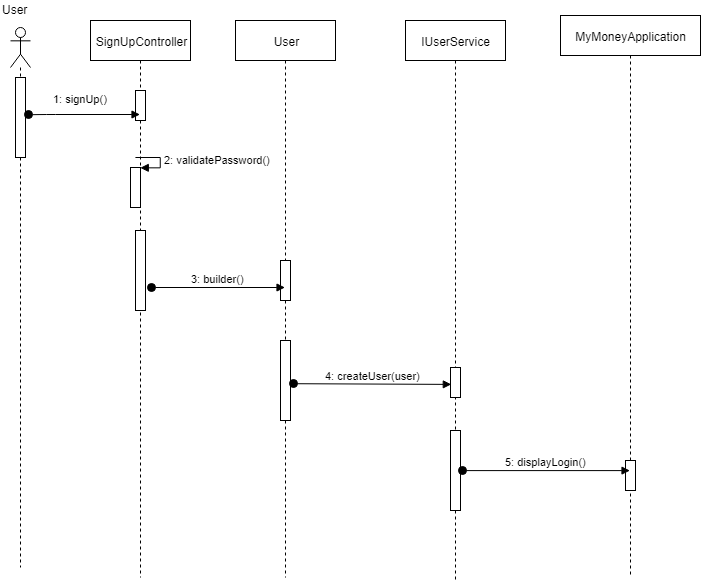
\includegraphics[width=\linewidth]{case1SequenceDiagram.png}
\caption{Use case 1 Sequence Diagram}
\label{fig:use-case-1-sequence-diagram}
\end{figure}

\clearpage

\subsubsection{Use Case 3: Add Bank Account to a User Account}

The following scenario describes the actions that occur when a user clicks the add button in the account list view.

\begin{figure}[H]
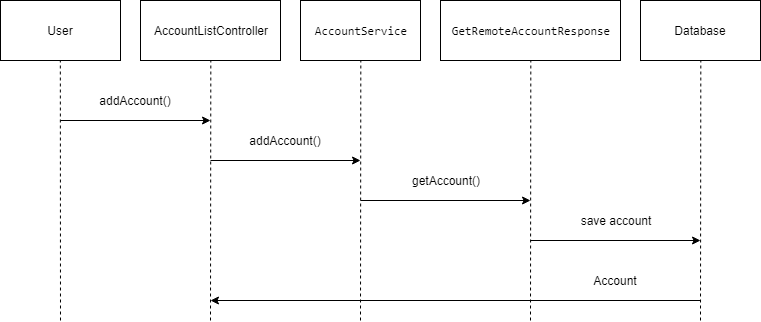
\includegraphics[width=\linewidth]{usecase3_sequence_diagram.png}
\caption{Use case 3 Sequence Diagram}
\label{fig:use-case-3-sequence-diagram}
\end{figure}

\clearpage

\subsubsection{Use Case 5: View Transactions for Specific Bank Account}

The following scenario describes the actions that occur when the user clicks the button<view transactions> for a specific bank account.

\begin{figure}[H]
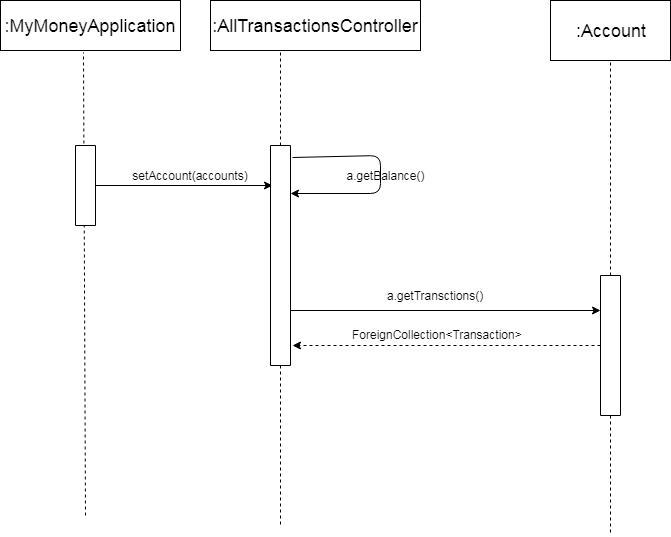
\includegraphics[width=\linewidth]{usecase5.png}
\caption{Use case 5 Sequence Diagram}
\label{fig:use-case-5-sequence-diagram}
\end{figure}

\clearpage

\clearpage

\subsubsection{Use Case 6: View All Transactions from all Bank Accounts}

The following scenario describes the actions that occur when the user click the button "view all transactions" for viewing all transactions from all bank accounts.

\begin{figure}[H]
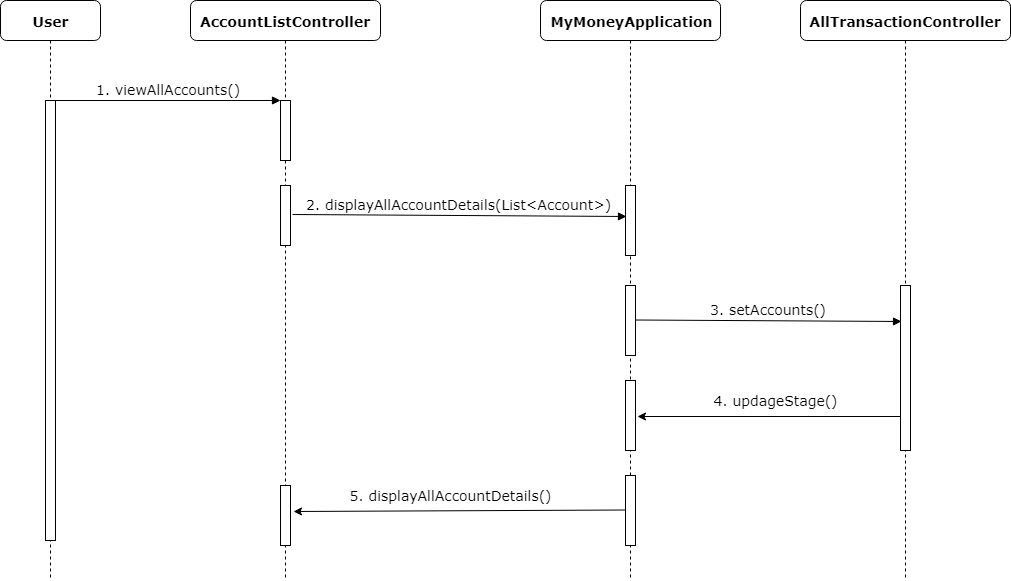
\includegraphics[width=\linewidth]{Use_Case_6_Sequence_Diagram.png}
\caption{UseCase 6 Sequence Diagram}
\label{fig:use-case-6-sequence-diagram}
\end{figure}

\clearpage

\section{Reference}

\begin{itemize}
\item User information: As our user and use-cases was based on feedback provided by our developers, our references lie mainly within our own team.
\item Craig Larman - Applying UML and Patterns
\item Greg Butler's course COMP 354 content
\item \href{http://web.mit.edu/ssit/cis/CISRequirements.html}{\textcolor{blue}{MIT Curricular Information System
Software Requirements Document}}
\item \href{https://resources.sei.cmu.edu/asset_files/TechnicalReport/2005_005_001_14621.pdf}{\textcolor{blue}{Carnegie Mellon Business Goals}}
\item \href{http://www.oracle.com/technetwork/testcontent/gettingstartedwithusecasemodeling-133857.pdf}{\textcolor{blue}{Use-Case: Oracle }}
\item \href{https://github.com/google/dagger}{\textcolor{blue}{Google Dagger Github}}

\end{itemize}

\end{document}
